\chapter{التطبيق خطوة بخطوة}
\label{ch:01b-build}

\section{ما الذي سنطبّقه؟}
\label{sec:build-start}

لنفترض أن لدينا مؤسسة اسمها «وزارة الاقتصاد والصناعة»، وتريد تنظيم الكشف على المنشآت التجارية. يكلّف أحمد الباحث نور بالكشف على «فرن الأمانة». يسجل نور نتيجة الزيارة ويرسلها إلى ريم للتدقيق. تعتمد ريم الكشف، أو تعيده لاستكمال النواقص، أو ترفضه مع توضيح السبب.

سنجهز هذا العمل بالترتيب: الفريق، ثم ملف المنشأة، ثم استمارة الكشف، ثم الموافقة والتكليف، ثم لوحة مؤشرات نبحث فيها عن المنشآت ونصفي نتائجها. تحتاج خطوات الإعداد إلى حساب مسؤول، أما تنفيذ الكشف فيكون بحساب الباحث والمدقق.

\begin{table}[H]
\centering
\caption{فريق المثال}
\label{tab:team}
\begin{tabularx}{\linewidth}{R{4cm} R{4cm} Y}
\rcHeaderRow
\thh{الشخص} & \thh{منصبه} & \thh{عمله في العملية}\\
أحمد سالم — تجريبي & رئيس فريق الكشف الميداني — 01 & يجهّز التكليف ويتابع إنجازه.\\
نور حسن — تجريبي & باحث ميداني — 01 & يزور المنشأة ويعبئ الكشف.\\
ريم خالد — تجريبي & مدقق كشوف المنشآت — 01 & تراجع الكشف وتتخذ القرار.\\
\end{tabularx}
\end{table}

\textbf{النتيجة:} تعرف الآن من سيعمل، وعلى أي منشأة، وما القرار الذي ينتهي به الكشف.

\section{أنشئ مكان الفريق في الهيكل}
\label{sec:build-nodes}

\textbf{لماذا؟} يحتاج النظام إلى معرفة الدائرة التي يعمل فيها الفريق. «الوحدة التنظيمية» هي مديرية أو دائرة داخل المؤسسة، وليست حساب موظف.

\begin{enumerate}
\item افتح «الموارد البشرية» ← «الوحدات التنظيمية» ← «سجل جديد». أنشئ «الإدارة العامة للتجارة الداخلية وحماية المستهلك» برمز \en{MEI-DIT} ونوع «إدارة عامة».
\item أنشئ «مديرية حماية المستهلك وسلامة الغذاء» برمز \en{DIT-CPSF} ونوع «مديرية»، واختر الإدارة العامة في «يتبع ل»، ثم اضغط «إنشاء».
\item أنشئ «دائرة حماية المستهلك» برمز \en{DIT-CPSF-CP} ونوع «دائرة»، واختر المديرية في «يتبع ل»، ثم اضغط «إنشاء».
\end{enumerate}

الرمز معرّف قصير يميّز الوحدة عندما تتشابه الأسماء. أما «يتبع ل» فيحدد الوحدة الأعلى منها.

\textbf{تحقق:} افتح دائرة حماية المستهلك؛ يجب أن تظهر مديرية حماية المستهلك وسلامة الغذاء في العلاقة «يتبع ل». إذا لم تظهر، عد إلى تعديل الدائرة وحدد المديرية.

\section{أنشئ الوظائف والمناصب}
\label{sec:build-positions}

\textbf{لماذا؟} «باحث ميداني» وصف للعمل المطلوب. أما «باحث ميداني — 01» فهو منصب محدد في دائرة حماية المستهلك. سنسند العمل إلى المنصب، ثم نحدد الشخص الذي يشغله.

\begin{table}[H]
\centering
\caption{أدخل هذه الأوصاف والمناصب}
\label{tab:positions}
\begin{tabularx}{\linewidth}{R{3cm} Y Y}
\rcHeaderRow
\thh{الوصف الوظيفي} & \thh{المنصب ورمزه} & \thh{المدير}\\
رئيس فريق الكشف الميداني & رئيس فريق الكشف الميداني — 01؛ \en{POS-CP-FIELD-LEAD-01} & رئيس دائرة حماية المستهلك.\\
باحث ميداني & باحث ميداني — 01؛ \en{POS-CP-INSPECTOR-01} & رئيس فريق الكشف الميداني — 01.\\
مدقق كشوف المنشآت & مدقق كشوف المنشآت — 01؛ \en{POS-CP-REVIEWER-01} & رئيس دائرة حماية المستهلك.\\
\end{tabularx}
\end{table}

\begin{enumerate}
\item افتح «الموارد البشرية» ← «وصف الوظيفة» ← «سجل جديد». أدخل أول مسمى من الجدول.
\item أدخل رمزه الوظيفي: \en{JD-CP-FIELD-LEAD} لرئيس الفريق، و\en{JD-CP-INSPECTOR} للباحث، و\en{JD-CP-REVIEWER} للمدقق. اضغط «إنشاء»، وكرر لكل وصف.
\item افتح «المناصب» ← «سجل جديد»، وأدخل اسم منصب رئيس الفريق ورمزه من الجدول.
\item اختر وصفه الوظيفي، واجعل «الوحدة» هي «دائرة حماية المستهلك»، وحدد «المدير»، ثم اضغط «إنشاء».
\item كرر للباحث والمدقق. أنشئ رئيس الفريق أولاً كي تتمكن من اختياره مديراً للباحث.
\end{enumerate}

\textbf{تحقق:} لكل منصب وصف ووحدة ومدير. انتبه إلى أن المدقق يتبع لرئيس الدائرة مباشرة، بينما الباحث يتبع لرئيس الفريق.

\section{أضف الأشخاص واربط كل شخص بمنصبه}
\label{sec:build-members}

\textbf{لماذا؟} المنصب يحدد المسؤولية، لكنه لا يحدد من يؤديها. «العضو» هو حساب الشخص، و«التعيين» هو الرابط بين هذا الحساب والمنصب؛ مثل تعيين نور في منصب الباحث.

\begin{enumerate}
\item افتح «الموارد البشرية» ← «الأعضاء» ← «سجل جديد».
\item أدخل «أحمد سالم — تجريبي» ورقم الموظف \en{DEMO-CP-001}، وبريده المخصص للعمل. اختر «مقعد كامل»، ثم اضغط «إنشاء».
\item كرر مع «نور حسن — تجريبي» برقم \en{DEMO-CP-002}، و«ريم خالد — تجريبي» برقم \en{DEMO-CP-003}، وبريد كل شخص.
\item افتح «التعيينات» ← «سجل جديد». اختر أحمد في «العضو»، و«رئيس فريق الكشف الميداني — 01» في «المنصب».
\item حدد تاريخ بدء عمله، واجعل الحالة «نشط»، ثم اضغط «إنشاء».
\item أنشئ تعيين نور في «باحث ميداني — 01»، وتعيين ريم في «مدقق كشوف المنشآت — 01» بالطريقة نفسها.
\end{enumerate}

\textbf{تحقق:} افتح «التعيينات»؛ يجب أن تجد ثلاثة تعيينات حالتها «نشط»، منها تعيين نور في «باحث ميداني — 01». إذا لم تجده، افتح التعيين وتأكد من العضو والمنصب والحالة. الخطوات التالية تعتمد على هذه التعيينات: الموافقة والتكليف يصلان إلى شاغل المنصب، لا إلى المنصب الفارغ.

\section{جهّز التطبيق وملف المنشأة}
\label{sec:build-entity}

\textbf{لماذا؟} نريد الاحتفاظ ببيانات كل منشأة مرة واحدة، ثم ربط كشوفها بها. «نوع السجلات» يشبه جدولاً: «المنشآت التجارية» هو الجدول، و«فرن الأمانة» سجل واحد فيه، و«العنوان التفصيلي» حقل داخل السجل. أما التطبيق فهو المكان الذي يجمع صفحات عمل الفريق.

\begin{enumerate}
\item افتح «ادوات البناء» ← «التطبيقات» ← «سجل جديد». اكتب العنوان «حماية المستهلك»، ووصفاً قصيراً لعمل الفريق، وأيقونة مثل \en{shield}، ثم اضغط «إنشاء».
\item افتح «أقسام التطبيق» ← «سجل جديد». اكتب «السجلات»، وأكمل الوصف والأيقونة، واختر تطبيق «حماية المستهلك»، ثم اضغط «إنشاء».
\item افتح «الكيانات» ← «إضافة كيان»، واكتب «المنشآت التجارية». الكيان هنا هو اسم آخر لنوع السجلات.
\item أضف الحقول الموضحة في الجدول. اضغط «إضافة حقل»، ثم اختر نوعه واكتب عنوانه، وكرر لكل حقل.
\item من «إعدادات الكيان»، اختر «اسم المنشأة» ضمن «حقول الاسم المعروض». بهذا يظهر اسم الفرن في القوائم بدلاً من معرّف غير مفهوم.
\item فعّل «إظهار في التنقل»، واختر التطبيق والقسم، ثم اضغط «انشاء كيان».
\item افتح «المنشآت التجارية» من التطبيق، واضغط «سجل جديد». أدخل «فرن الأمانة» وبياناته الفعلية، ثم احفظ السجل.
\end{enumerate}

\begin{table}[H]
\centering
\caption{الحقول الأساسية لملف المنشأة}
\label{tab:fields}
\begin{tabularx}{\linewidth}{R{4cm} R{2cm} Y}
\rcHeaderRow
\thh{الحقل} & \thh{نوعه} & \thh{فائدته}\\
اسم المنشأة & نص & الاسم الذي نختار به المنشأة؛ اجعله مطلوباً.\\
رقم السجل التجاري & نص & يحفظ الرقم كما هو، بما فيه الأصفار في بدايته.\\
النشاط & اختيار & يحدد نشاط المنشأة من قائمة موحدة.\\
المحافظة & اختيار & يحدد المحافظة من قائمة موحدة.\\
العنوان التفصيلي & نص & يحفظ وصف الوصول إلى المنشأة.\\
الموقع على الخريطة & موقع & يحفظ موضعها الجغرافي.\\
\end{tabularx}
\end{table}

\begin{figure}[H]
\centering
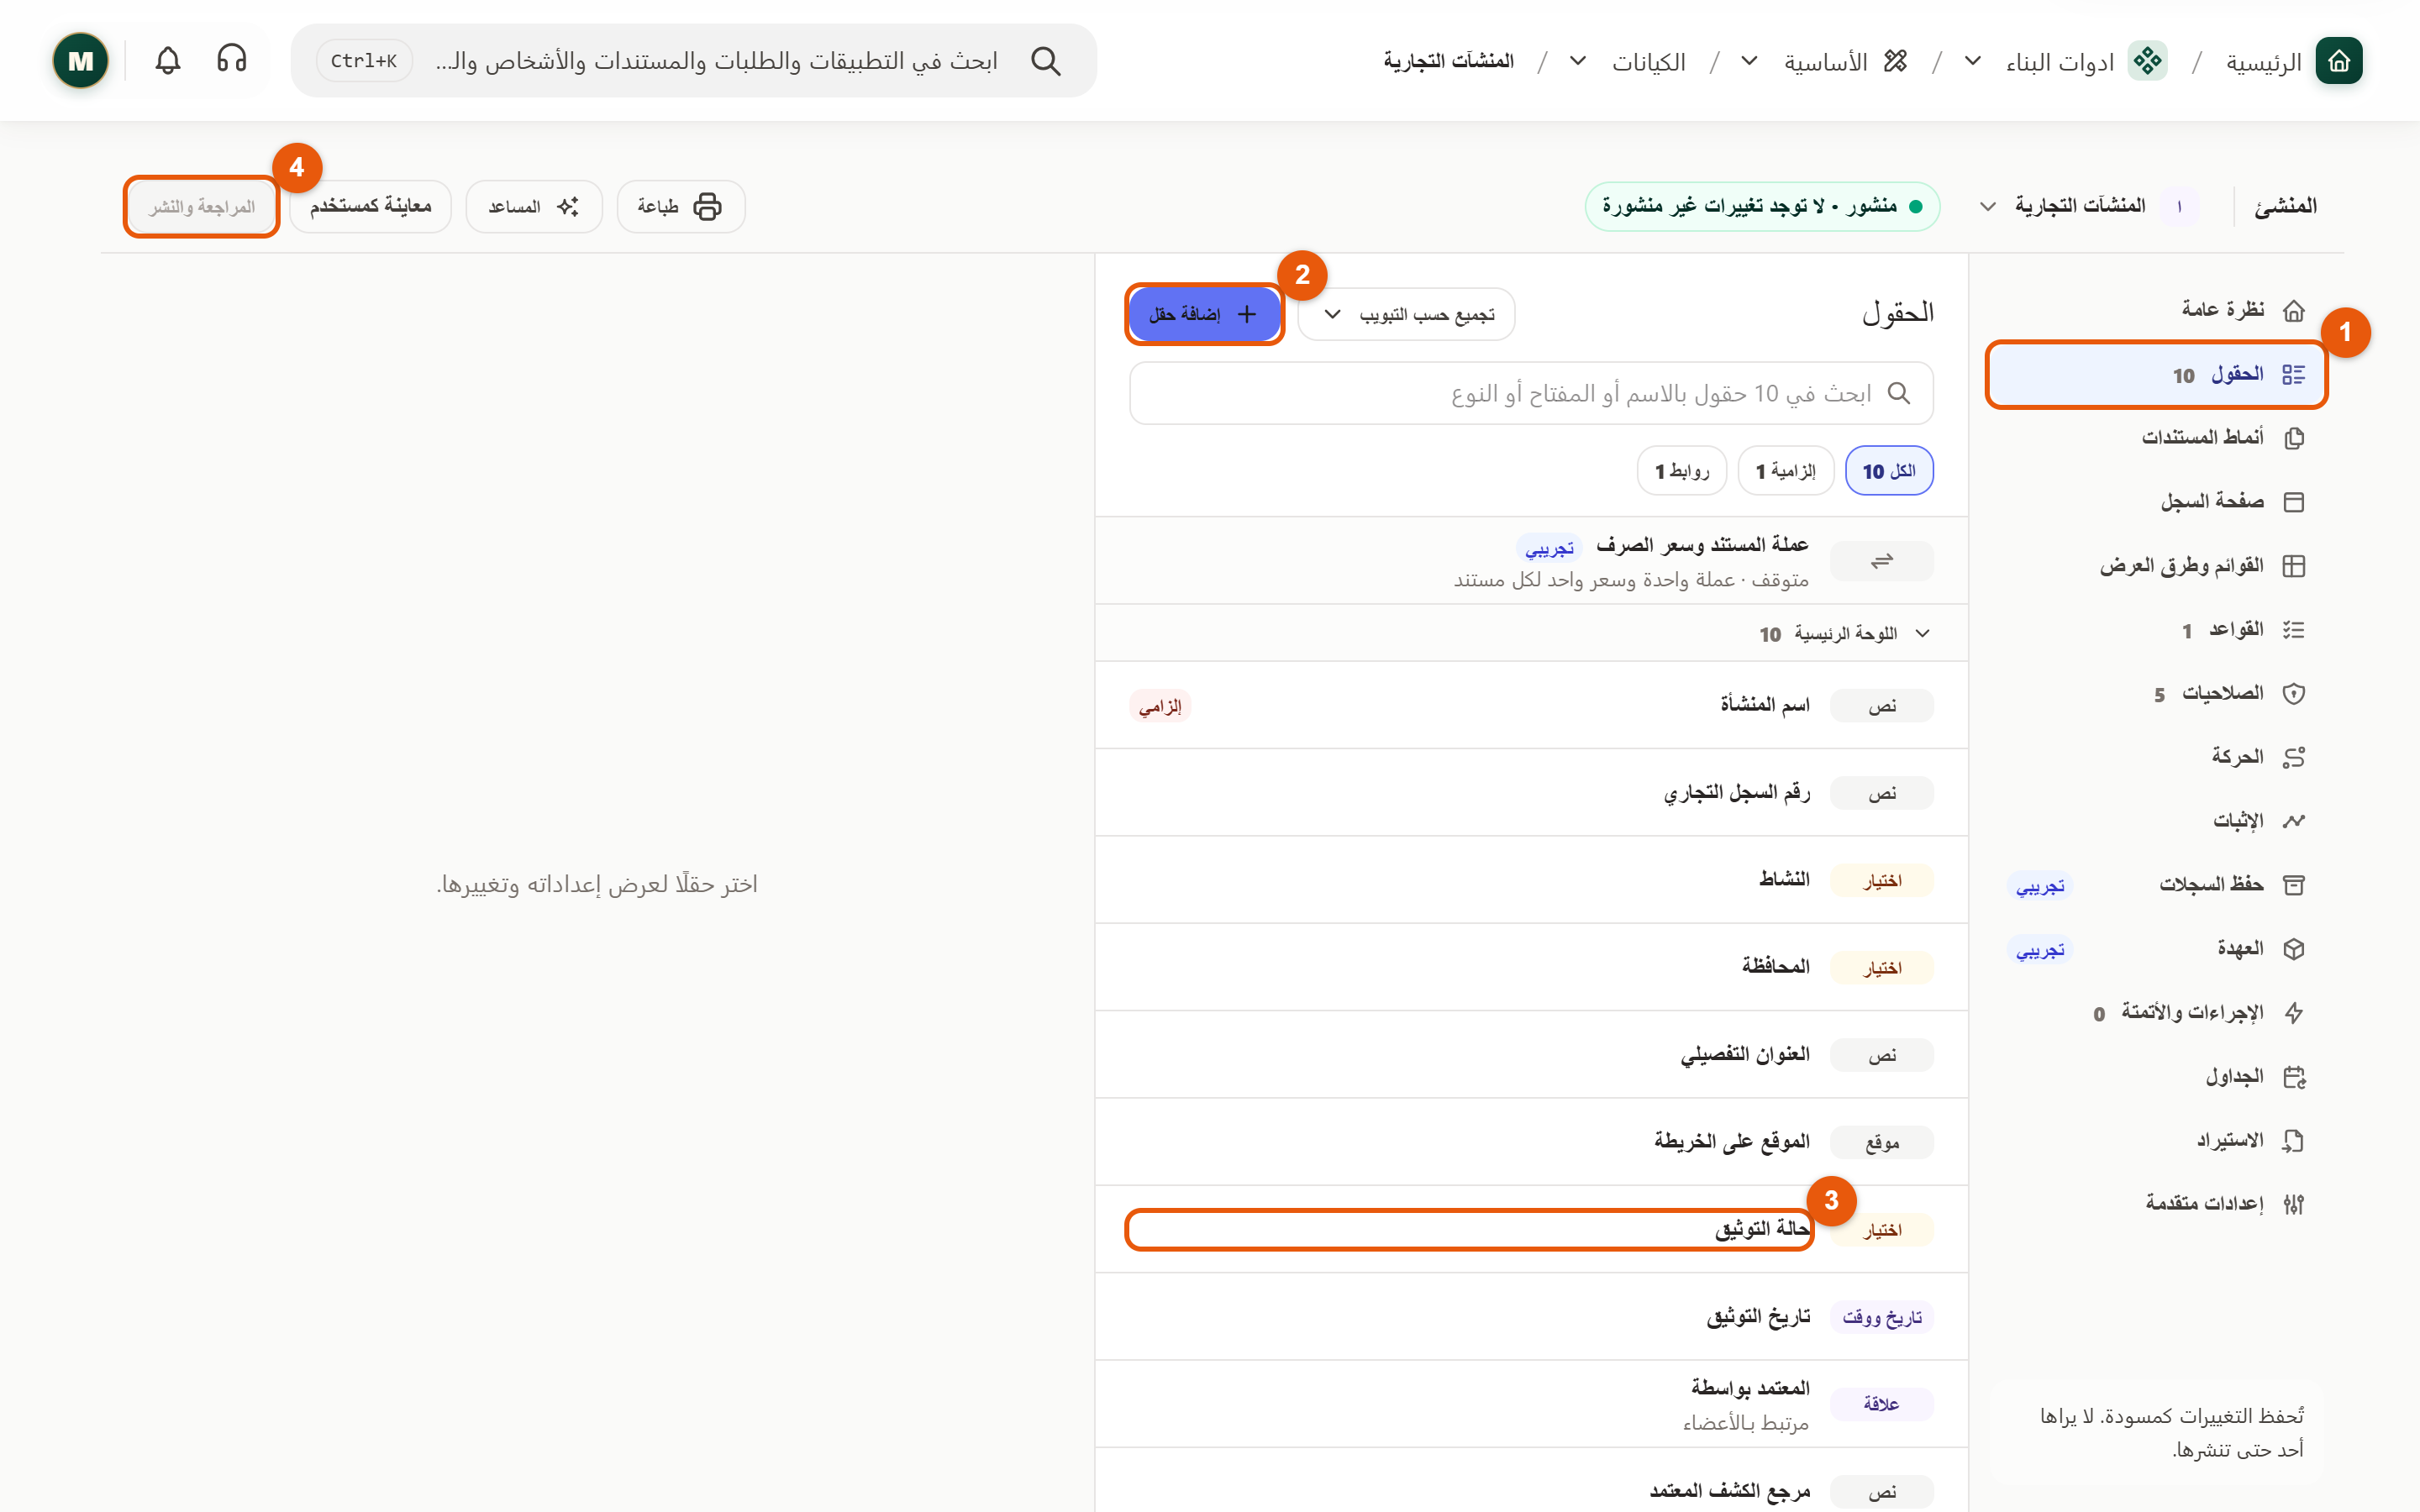
\includegraphics[width=0.95\linewidth]{assets/screens/entity-fields.png}
\caption{إعداد حقول المنشآت التجارية}
\label{fig:fields}
\shotnote{تجمع هذه الشاشة البيانات التي يحفظها ملف كل منشأة. ① «الحقول»: افتح قائمة الحقول. ② «إضافة حقل»: أضف معلومة جديدة. ③ «حالة التوثيق»: مثال لحقل إضافي، وليس حالة سير الكشف. ④ «المراجعة والنشر»: أتح التعديلات للمستخدمين.}
\end{figure}

\textbf{تحقق:} يظهر «فرن الأمانة» باسمه في القائمة، ويفتح ببياناته. إذا ظهر بمعرّف فقط، حدّد «اسم المنشأة» حقلاً للاسم المعروض.

\subsection{اضبط الحقول قبل استخدامها في النموذج واللوحة}

\begin{enumerate}
\item افتح حقل «اسم المنشأة»، وتأكد أن نوعه نص وأنه مطلوب. اسم الحقل يصف المعلومة، أما قيمته داخل أول سجل فهي «فرن الأمانة».
\item افتح حقل «المحافظة»، وأضف خيارات المحافظات التي يغطيها العمل. لكل خيار عنوان يراه المستخدم ومفتاح تحفظه البيانات. استخدم هذه الخيارات نفسها عند ربط سؤال المحافظة؛ لا تنشئ قائمة ثانية بمفاتيح مختلفة.
\item كرر للنشاط، مع خيار يصف نشاط الفرن. لا تجمع النشاط والمحافظة في حقل واحد؛ كل منهما سيكون محوراً مستقلاً للبحث والرسم.
\item اضبط العنوان التفصيلي كنص والموقع كحقل موقع. العنوان يشرح الوصول، والموقع يحدد النقطة؛ وجود أحدهما لا يملأ الآخر تلقائياً.
\item راجع حقول الاسم المعروض والتطبيق والقسم، ثم افتح «المراجعة والنشر» وانشر تعديلات الحقول قبل استخدامها في النموذج.
\item افتح سجل الفرن واملأ المحافظة والنشاط والعنوان والموقع. احفظ، ثم أعد فتحه للتأكد من بقاء القيم.
\end{enumerate}

\textbf{تحقق:} تستطيع اختيار المحافظة والنشاط من قوائم واضحة. احتفظ بمعنى الحقول ومفاتيحها عند تعديل التصميم لاحقاً؛ تغيير عنوان ظاهر يختلف عن حذف حقل يحمل بيانات أو تغيير نوعه.

\section{أنشئ استمارة الكشف}
\label{sec:build-form}

\textbf{لماذا؟} ملف المنشأة يحفظ معلوماتها الأساسية، أما «النموذج» فهو الاستمارة التي يملؤها الباحث في كل زيارة. يمكن أن يكون للمنشأة الواحدة عدة كشوف، ولكل كشف إجابات وقرار مستقلان.

\subsection{افهم ما الذي تبنيه قبل إضافة الأسئلة}

النموذج هو القالب، و«الإجابة» هي كشف واحد يعبئه نور باستخدام هذا القالب. القسم يرتب الأسئلة، والسؤال يجمع معلومة واحدة، والقاعدة تضبط متى يظهر السؤال أو متى تكون إجابته صحيحة. أما المسار فينظم ما يحدث بعد الإرسال. سنضبط هذه الأجزاء بالتتابع ثم نجربها معاً.

رتّب النموذج كما تحدث الزيارة: أولاً تحديد المنشأة وقراءة بياناتها، ثم تسجيل الملاحظات والتوصية، ثم إرفاق ما يدعمها. لا تضع سؤال المنشأة بعد الأسئلة المرتبطة به؛ فالباحث يحتاج اختيار الملف قبل مراجعة معلوماته.

\begin{enumerate}
\item افتح «ادوات البناء» ← «النماذج»، واضغط «إنشاء نموذج».
\item اكتب «كشف منشأة تجارية لطلب سجل تجاري»، والكود \en{001}، واختر تطبيق «حماية المستهلك» وقسم «السجلات»، ثم اضغط «إنشاء». وإذا طلب اختصاراً مرجعياً، أدخل اختصاراً يستخدم لترقيم الكشوف؛ وهو مختلف عن كود النموذج.
\item قسّم الاستمارة إلى بيانات المنشأة، ونتيجة الكشف، والمرفقات. القسم يجمع أسئلة مرتبطة ليسهل على الباحث تعبئتها.
\item أضف أسئلة نتيجة الزيارة: اختر نوع «نص» للملاحظات، ونوع الاختيار للتوصية، ونوع الملفات للمرفقات. اكتب عنواناً يوضح للباحث ما المطلوب في كل سؤال.
\item اجعل المعلومات الضرورية مطلوبة، ثم انتقل إلى الخطوة التالية لربط الاستمارة بالمنشأة.
\end{enumerate}

\begin{figure}[H]
\centering
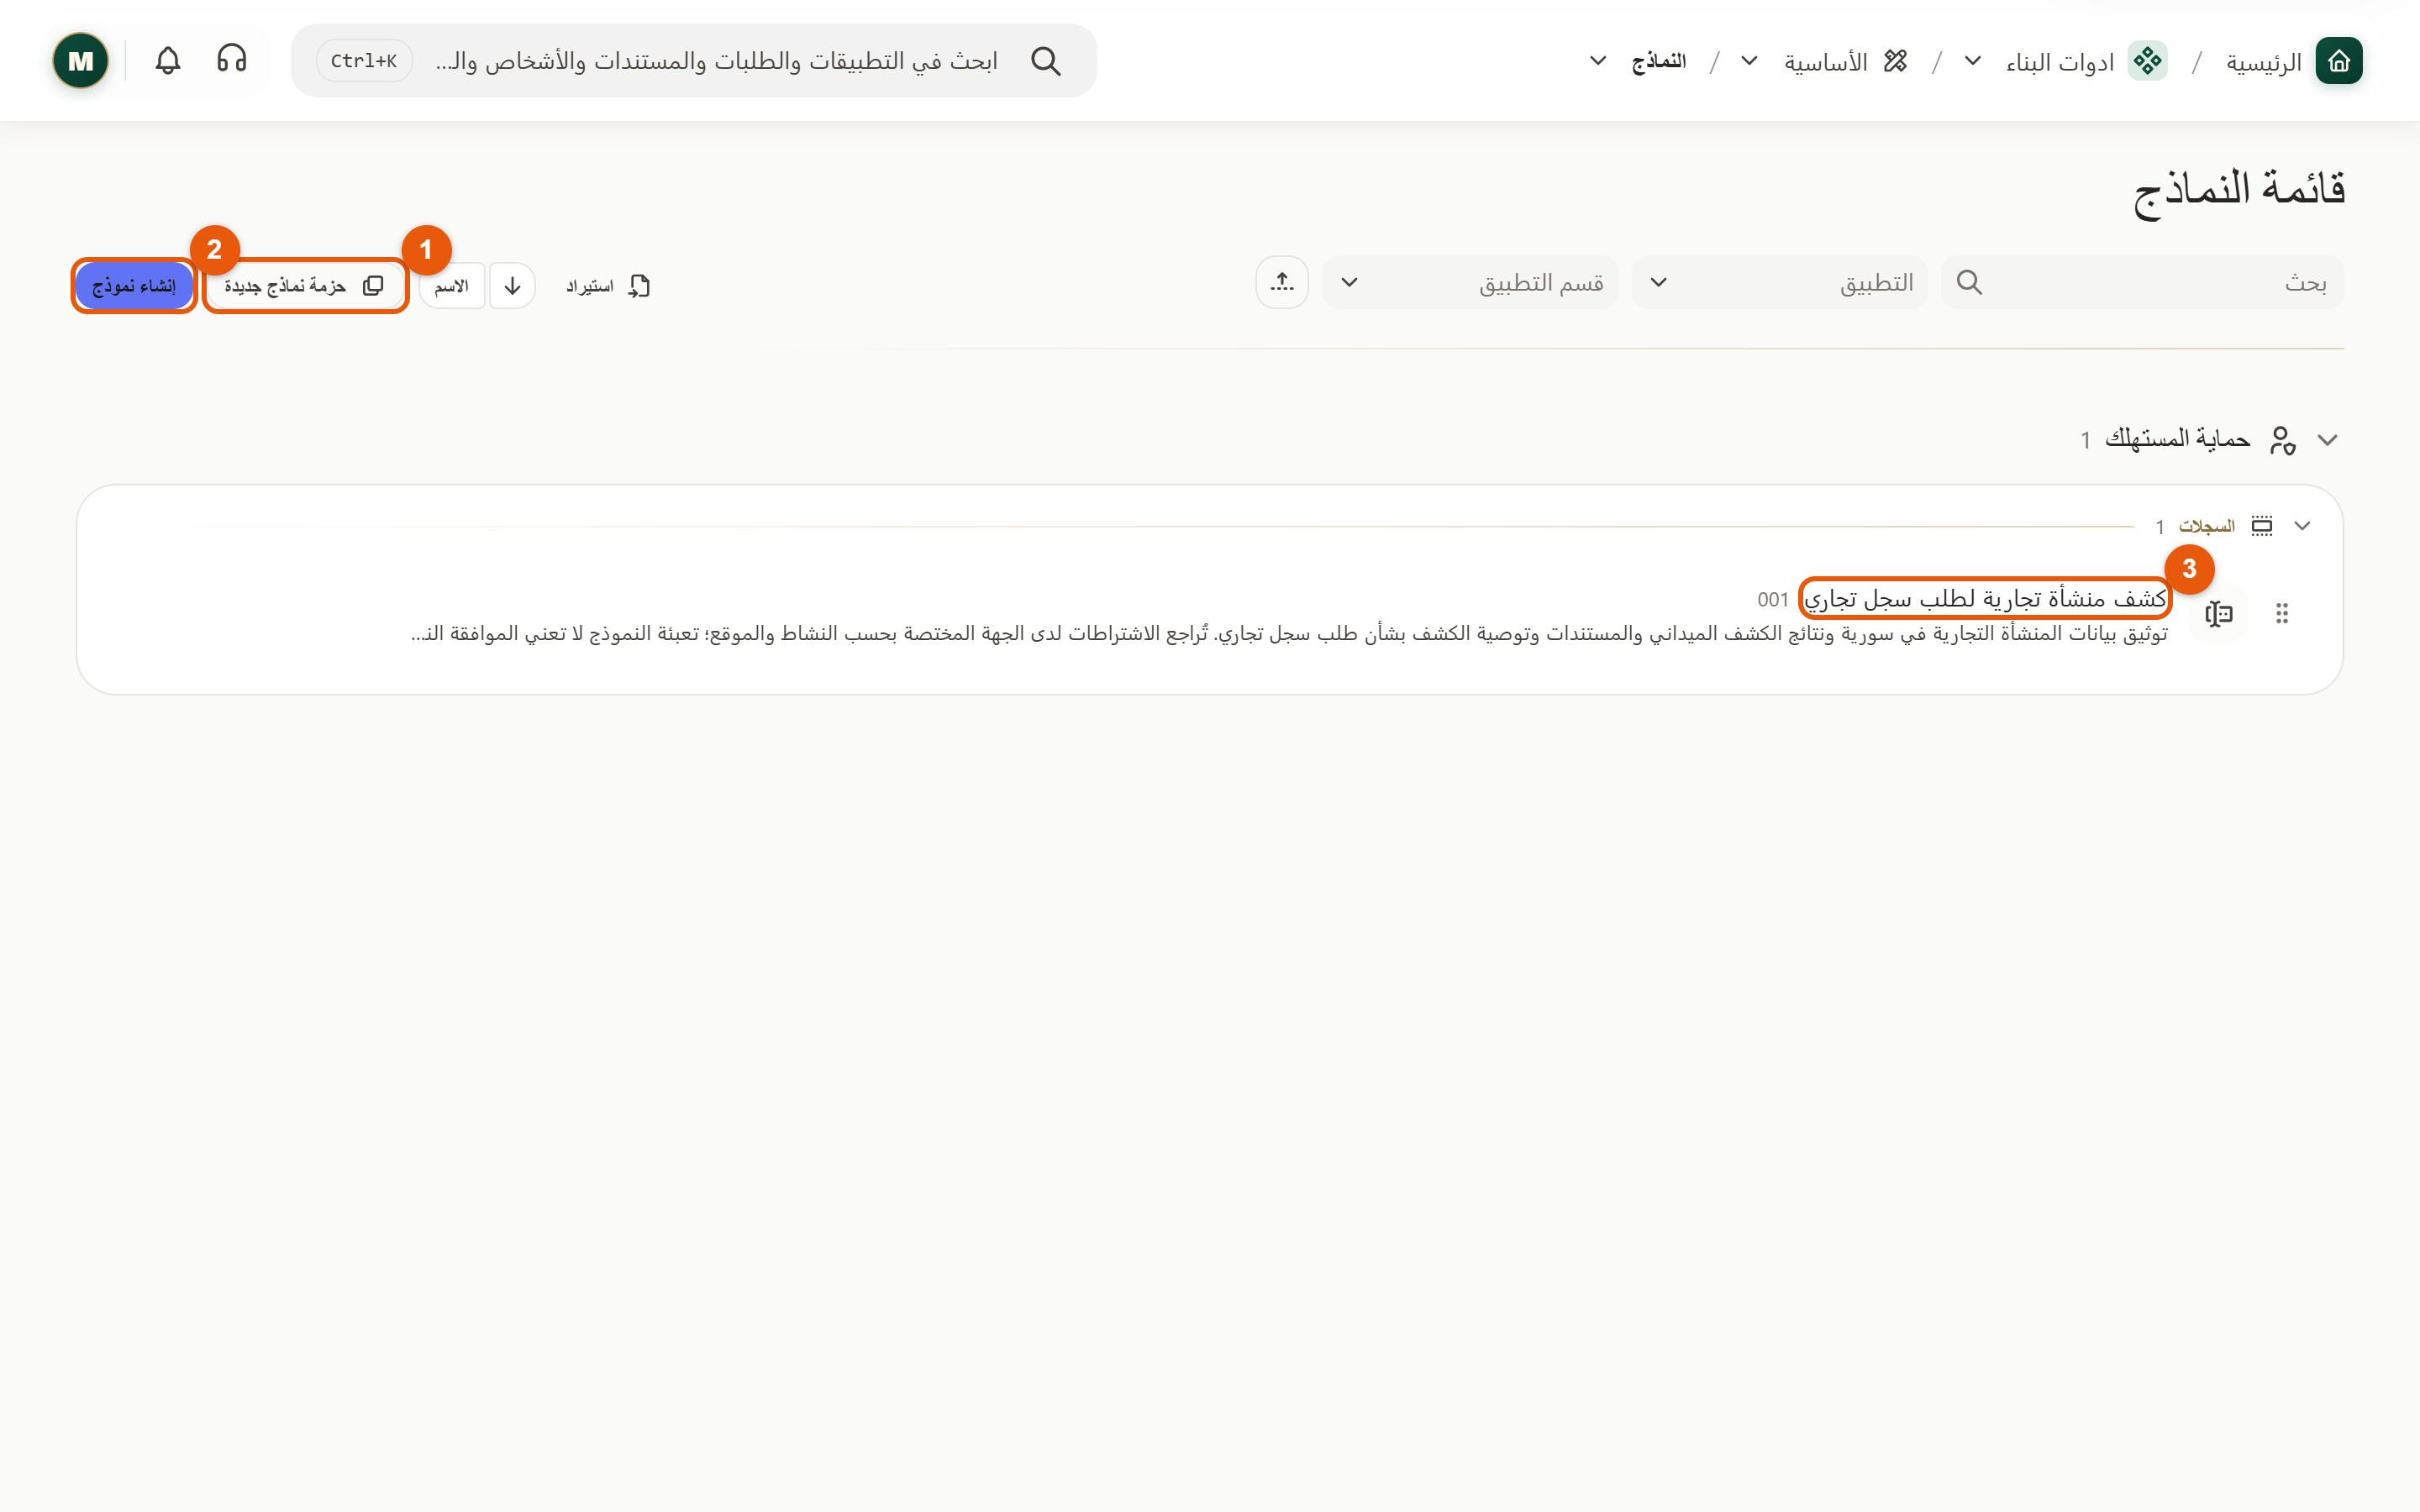
\includegraphics[width=0.95\linewidth]{assets/screens/forms-list.png}
\caption{إنشاء نموذج الكشف}
\label{fig:forms}
\shotnote{تبدأ الاستمارة من قائمة النماذج، ثم تفتح في المحرر. ① «حزمة نماذج جديدة»: تجمع عدة نماذج؛ لا نحتاجها لهذا الكشف الواحد. ② «إنشاء نموذج»: ابدأ استمارة الكشف. ③ نموذج المثال باسمه وكوده.}
\end{figure}

\textbf{تحقق:} يظهر عنوان الكشف في المحرر، وتظهر تحته الأقسام والأسئلة. لم يصل النموذج إلى الفريق بعد؛ سننشره بعد ضبط الربط والموافقة.

\subsection{ابنِ الأقسام والأسئلة واحداً واحداً}

\begin{enumerate}
\item أضف القسم الأول وسمّه «بيانات المنشأة». اكتب وصفاً قصيراً: «اختر المنشأة ثم راجع بياناتها وصحح ما تغير». سنضيف إليه سؤال السجل والأسئلة المرتبطة في الخطوتين التاليتين.
\item أضف قسم «نتيجة الكشف». من شريط إضافة الأسئلة افتح «اختر نوع الحقل» واختر سؤالاً نصياً. هذا الزر يضيف سؤالاً جديداً؛ تأكد أنك لا تضيف سؤالاً ثانياً عندما تريد تعديل الأول.
\item حدّد السؤال المضاف واكتب عنوانه «ملاحظات الكشف». في وصفه اكتب ما يفيد الباحث: «دوّن ما شاهدته في الزيارة وما يحتاج إلى تصحيح». العنوان اسم المعلومة؛ والوصف يشرح طريقة الإجابة عنها.
\item أضف سؤال اختيار باسم «توصية القائم بالكشف». أضف خياراً للتوصية بالموافقة، ثم ثلاثة خيارات سنستخدمها في قاعدة لاحقة: «استكمال نواقص قبل البت»، و«الحاجة إلى إعادة كشف»، و«عدم التوصية بالموافقة مع بيان الأسباب». استخدم اختياراً واحداً لأن الكشف يحتاج توصية واحدة، واجعله مطلوباً. توصية الباحث لا تعتمد الكشف تلقائياً؛ القرار يبقى لريم.
\item أضف قسم «المرفقات»، ثم سؤال ملفات يطلب صور الكشف أو مستنداته. اكتب في الوصف ما يجب تصويره أو إرفاقه. لا تجعل رفع الملف إلزامياً إلا إذا كانت إجراءات الكشف تتطلبه لكل زيارة.
\item راجع ترتيب الأسئلة داخل الأقسام. في المعاينة يجب أن يفهم الباحث ما المطلوب من العنوان والوصف دون سؤال مسؤول النظام.
\end{enumerate}

\subsection{اضبط السؤال: النوع والمطلوب والتكرار}

لنضبط سؤال «رقم التواصل» مثالاً على إعداد نوع السؤال. حدده في الاستمارة، ثم اتبع الأرقام في الصورة: اختر نوعه من ①، واضبط عرضه من ②، واجعل صيغته «رقم هاتف» عند ③ ورمز الدولة عند ④، ثم افتح «القواعد» عند ⑤. العرض يغيّر مساحة السؤال، بينما الصيغة تحدد شكل الإجابة المقبولة.

\begin{figure}[H]
\centering
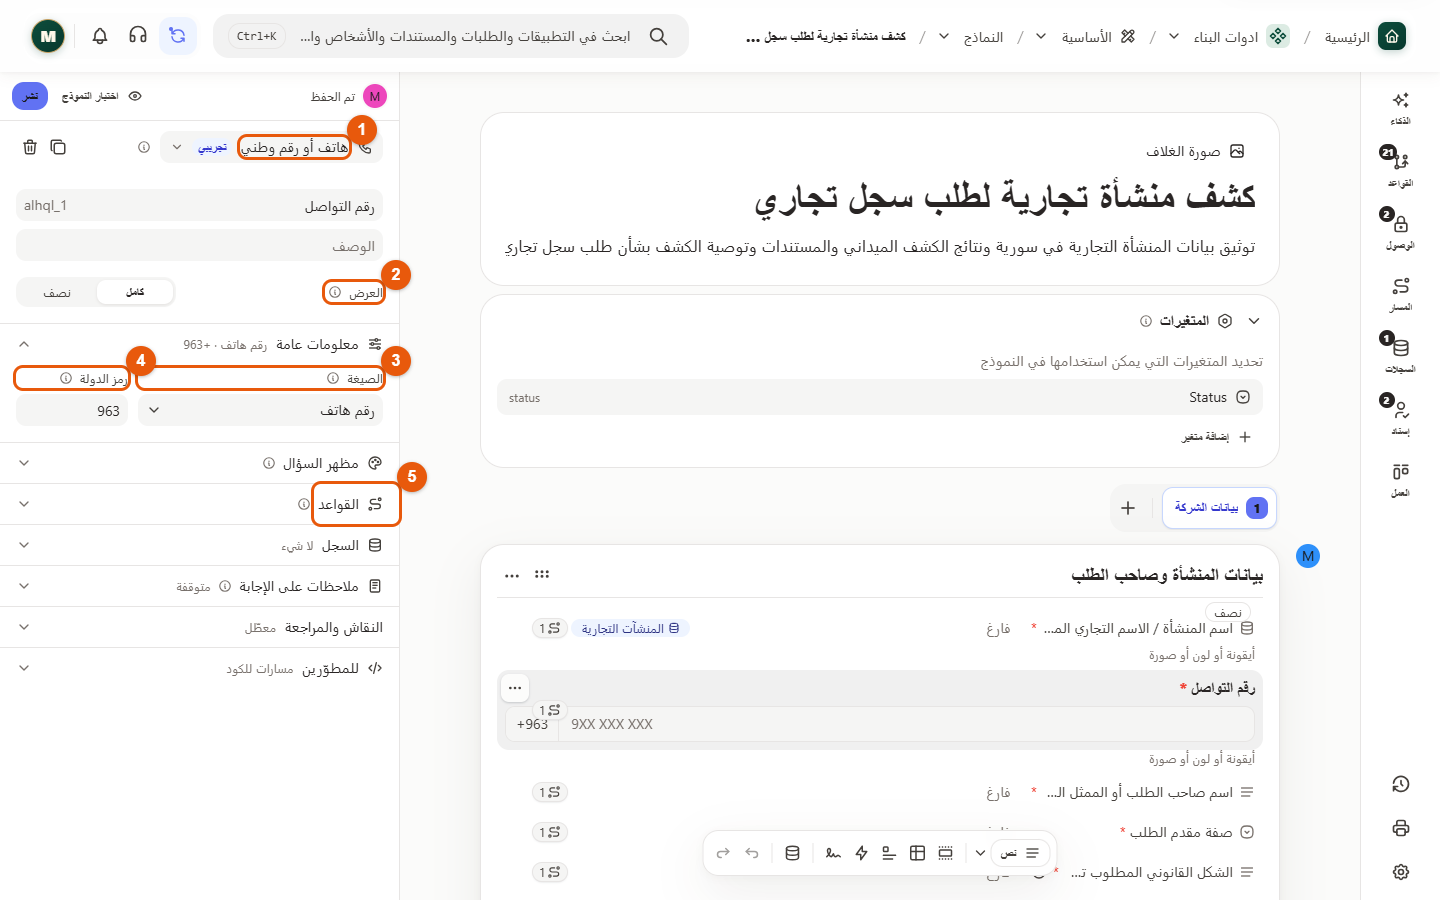
\includegraphics[width=0.95\linewidth]{assets/screens/org-question-settings.png}
\caption{إعداد نوع سؤال التواصل وعرضه وصيغته}
\label{fig:question-settings}
\shotnote{① نوع السؤال «هاتف أو رقم وطني». ② العرض: كامل أو نصف. ③ الصيغة: «رقم هاتف» لهذا السؤال. ④ رمز الدولة. ⑤ افتح قواعد السؤال لضبط الإلزام والظهور والتعديل.}
\end{figure}

\begin{table}[H]
\centering
\caption{قرارات تتخذها عند إعداد كل سؤال}
\label{tab:question-settings}
\begin{tabularx}{\linewidth}{R{3cm} Y Y}
\rcHeaderRow
\thh{الإعداد} & \thh{معناه} & \thh{قرارنا في الكشف}\\
نوع السؤال & يحدد شكل الإجابة وطريقة التحقق منها. & نص للملاحظات، اختيار للتوصية، ملفات للأدلة، وسجل لاختيار المنشأة.\\
مطلوب & يمنع الإرسال إذا غابت الإجابة المطلوبة. & فعّله للمنشأة والتوصية؛ لا تفعّله لكل شيء بلا سبب.\\
مقفل & يعرض القيمة دون أن يعدّلها الباحث. & استخدمه لمعلومة للعرض فقط، مع مصدر يملؤها. لا تقفل سؤالاً مطلوباً وفارغاً.\\
متكرر & يسمح بمجموعة إجابات للسؤال بدلاً من قيمة واحدة. & اتركه متوقفاً للأسئلة المرتبطة بحقل واحد كالمحافظة والعنوان.\\
القيمة الافتراضية & تعطي قيمة ابتدائية قبل إدخال الباحث. & لا تفترض توصية بالموافقة؛ دع الباحث يختار نتيجة زيارته.\\
قاعدة تحقق & تفحص صحة الإجابة، وليس مجرد وجودها. & استخدمها عندما توجد قاعدة عمل محددة، مع رسالة توضح التصحيح المطلوب.\\
\end{tabularx}
\end{table}

بعد فتح «القواعد»، اتبع ① لتحديد هل الإجابة مطلوبة، و② لظهور السؤال، و③ للسماح بتعديله. راجع ④ قبل وضع قيمة تلقائية، واترك ⑤ متوقفاً عندما تريد إجابة واحدة، واستخدم ⑥ لإضافة شرط صحة الإجابة.

\begin{figure}[H]
\centering
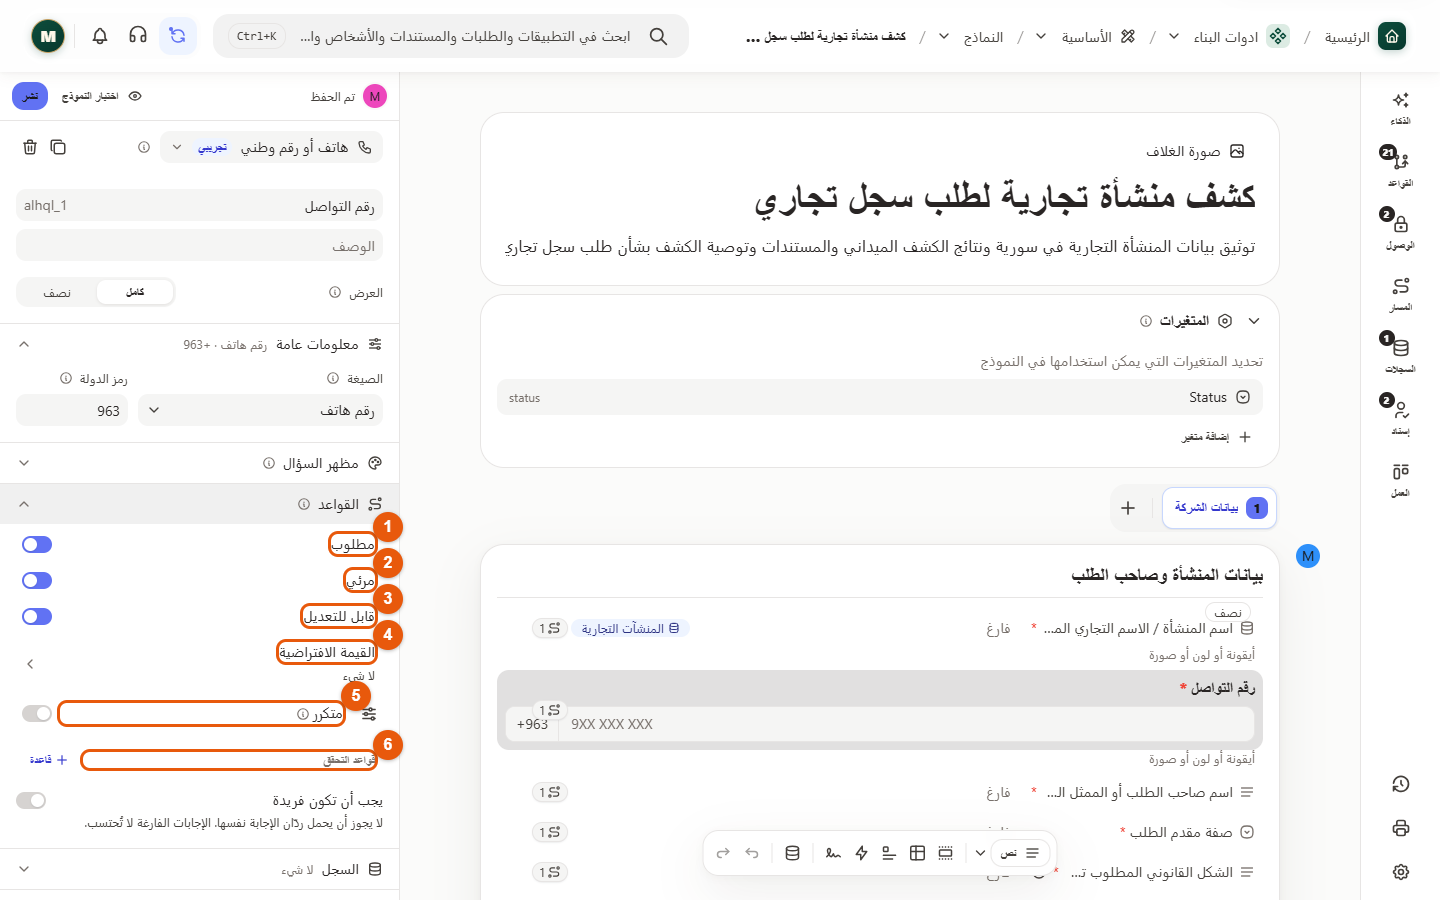
\includegraphics[width=0.95\linewidth]{assets/screens/org-question-rules.png}
\caption{قواعد السؤال: الإلزام والظهور والتعديل والقيمة الافتراضية}
\label{fig:question-rules}
\shotnote{① «مطلوب»: لا تترك الإجابة فارغة. ② «مرئي»: يظهر السؤال للباحث. ③ «قابل للتعديل»: إيقافه يقفل تعديل الإجابة. ④ «القيمة الافتراضية»: مصدر القيمة الأولية. ⑤ «متكرر»: أكثر من إجابة للسؤال. ⑥ «قواعد التحقق»: شروط صحة الإجابة.}
\end{figure}

الاختيار يختلف عن النص: قائمة المحافظات تمنع كتابة الاسم بعدة صيغ، فتستطيع اللوحة جمع المنشآت تحت محافظة واحدة. والرقم يختلف عن المعرّف: رقم السجل التجاري نحفظه كنص لأننا لن نجمعه حسابياً، ولأن الصفر في بدايته قد يكون مهماً.

\textbf{تحقق:} افتح «اختبار النموذج»، واترك التوصية فارغة ثم حاول الإرسال. يجب أن يوضح النموذج السؤال المطلوب. أكمله وتأكد من زوال التنبيه. جرّب إدخال الملاحظات ورفع مرفق وفتحه، ولا تكتفِ بظهور السؤال في المحرر.

\subsection{قواعد الظهور والإلزام: متى نحتاجها؟}

قاعدة الظهور تجيب: متى يحتاج الباحث هذا السؤال؟ وقاعدة الإلزام تجيب: متى يجب أن يجيب عنه؟ مثلاً عند التوصية بالرفض نحتاج تفسيراً، بينما قد لا نحتاجه بالطول نفسه عند التوصية بالموافقة. الإخفاء ليس وسيلة لحماية بيانات سرية؛ الصلاحيات هي التي تحدد الوصول.

\begin{enumerate}
\item في قسم «نتيجة الكشف»، أضف سؤالاً نصياً بعنوان «أسباب التوصية والنواقص المطلوب استكمالها»، ثم افتح «القواعد» وأضف قاعدة من نوع «إلزام» عند ① في الصورة. اختر «مطلوب عندما».
\item اختر «أيّ» عند ②. أضف عند ③ ثلاثة شروط على سؤال «توصية القائم بالكشف»: «استكمال نواقص قبل البت»، أو «الحاجة إلى إعادة كشف»، أو «عدم التوصية بالموافقة مع بيان الأسباب». يكفي تحقق واحدة منها لإلزام السبب.
\item عند «ثم ألزم» ④ اختر سؤال «أسباب التوصية والنواقص المطلوب استكمالها»، ثم اضغط «حفظ في المسودة» ⑤. اترك السؤال ظاهراً؛ نحن نغيّر وجوب الإجابة فقط.
\item إذا أردت إظهار سؤال عند حالة محددة، اضبط قاعدة الظهور لذلك السؤال ثم جرّب الفرعين: حالة يتحقق فيها الشرط وحالة لا يتحقق فيها. افحص الإلزام أيضاً حتى لا تمنع إجابة مخفية إرسال الكشف.
\item في «اختبار النموذج» اختر «عدم التوصية بالموافقة مع بيان الأسباب»، واترك سؤال الأسباب فارغاً، ثم جرّب الإرسال. يجب أن يمنعك النموذج ويشير إلى سؤال الأسباب. اكتب السبب وأعد المحاولة. غيّر التوصية وتأكد من أن القاعدة تتبع الاختيار الجديد.
\end{enumerate}

\begin{figure}[H]
\centering
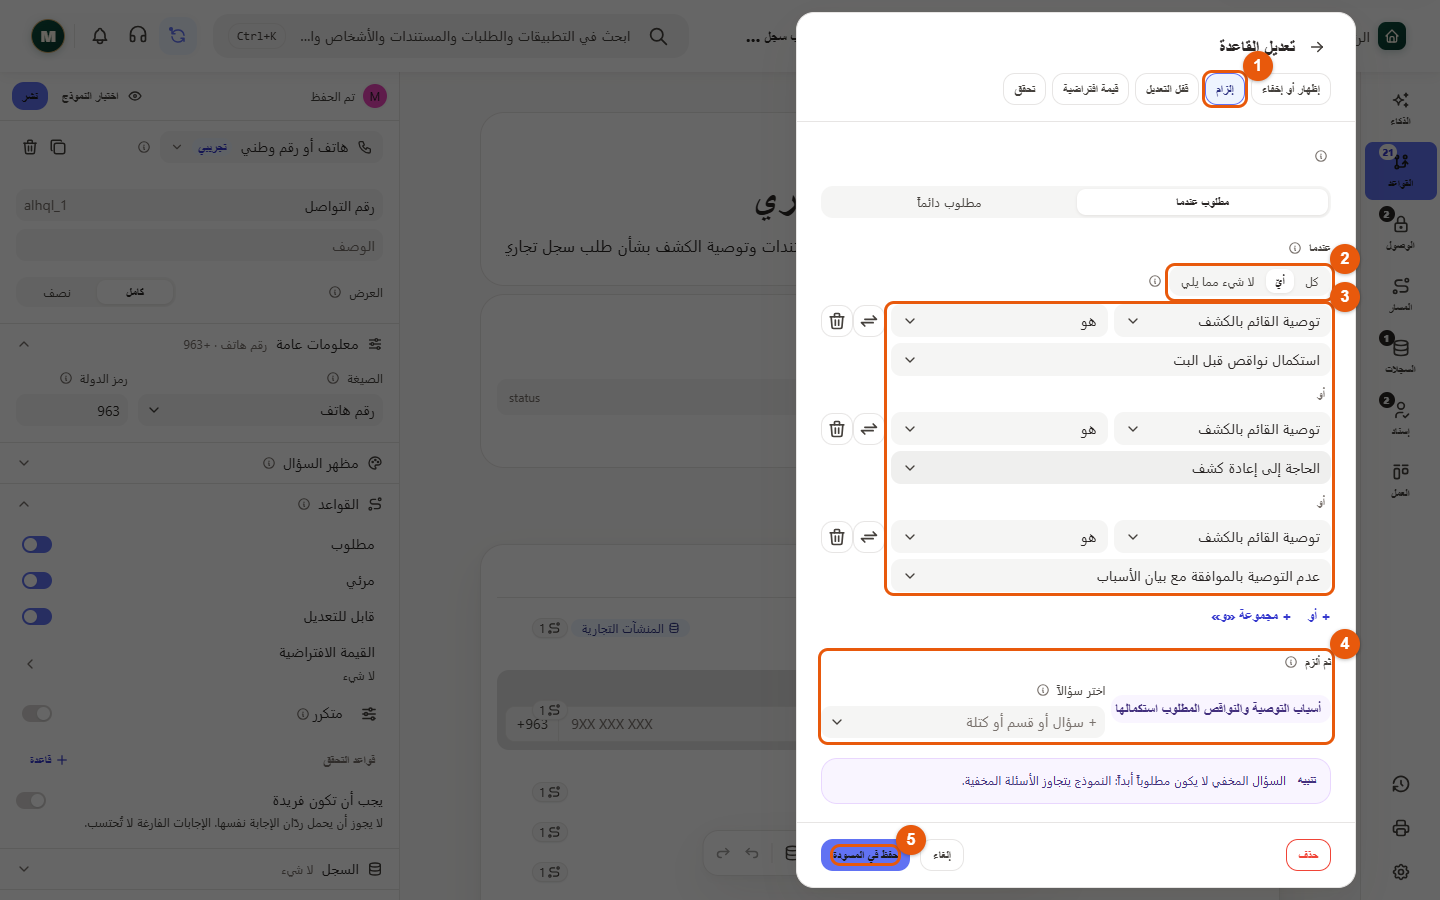
\includegraphics[width=0.95\linewidth]{assets/screens/org-required-condition.png}
\caption{إلزام أسباب التوصية عند الاستكمال أو إعادة الكشف أو عدم الموافقة}
\label{fig:required-condition}
\shotnote{① نوع القاعدة «إلزام». ② «أيّ»: تحقق واحد من الشروط يكفي. ③ شروط التوصية الثلاثة المتصلة بـ«أو». ④ السؤال الذي يصبح مطلوباً عند تحقق الشرط. ⑤ حفظ القاعدة في المسودة، ثم اختبارها قبل نشر النموذج.}
\end{figure}

\textbf{تحقق:} جرّب كل توصية من الثلاث دون سبب ثم مع سبب. يجب أن يصبح سؤال الأسباب مطلوباً في كل منها. السؤال المخفي يتجاوزه النموذج ولا يكون مطلوباً؛ لذلك أبقِ سؤال الأسباب ظاهراً في هذه القاعدة.

\subsection{القيم الافتراضية والمتغيرات دون خلطها بالربط}

القيمة الافتراضية قيمة بداية؛ أما قراءة حقل المنشأة فتأتي من الملف الذي اختاره الباحث. لذلك لا تكتب عنوان الفرن كقيمة ثابتة: اربطه بحقل العنوان ليعمل النموذج مع أي منشأة. والمتغير قيمة محسوبة أو مساعدة تستخدمها القواعد؛ لا تحتاج إلى إنشاء متغير لكل سؤال أو لكل حقل مرتبط.

عند استخدام محرر تعبيرات لقيمة ثابتة، يكتب النص بين علامتي تنصيص مثل \en{"KSHF"}، بينما يكتب العدد كعدد. وفي سؤال الاختيار تكون القيمة مفتاح الخيار المحفوظ، وقد تختلف عن عنوانه العربي. انسخ المفتاح من إعداد الخيارات واقرأ «النتيجة» قبل الحفظ؛ لا تفترض مفتاحاً من عندك. وإذا أردت قيمة واحدة، تأكد من إيقاف «متكرر».

\textbf{تحقق:} لا يحمل النموذج توصية مسبقة بالموافقة، ولا عنواناً ثابتاً لمنشأة بعينها. أي قيمة تلقائية تعرف مصدرها: حقل مرتبط أو قاعدة واضحة.

\section{أضف «سؤال سجل»: أي منشأة سنكشف عليها؟}
\label{sec:build-record-question}

\textbf{ما معنى سؤال سجل؟} هو سؤال يتيح اختيار سجل من النوع الذي أنشأناه. في هذا المثال يختار الباحث «فرن الأمانة»، الذي أضفناه في خطوة تجهيز ملف المنشأة. يحفظ النظام رابطاً إلى ملف الفرن، وليس مجرد كتابة اسمه كنص.

\textbf{لماذا نحتاجه؟} لو كتب الباحث اسم الفرن في سؤال نصي، فلن يعرف النظام أي ملف منشأة يقصده. سؤال السجل هو الذي يربط الكشف بالملف الصحيح، ويسمح بجلب بياناته وتحديث الحقول المرتبطة به لاحقاً.

\begin{enumerate}
\item داخل محرر النموذج، اضغط «السجلات» في الشريط الجانبي.
\item اضغط «سؤال سجل» عند العلامة ① في الصورة.
\item اختر «المنشآت التجارية» في «نوع السجل». هذا يحدد القائمة التي سيختار الباحث منها.
\item سمِّ السؤال «اسم المنشأة / الاسم التجاري المقترح»، واجعله مطلوباً. اختر «موجود فقط» كي يختار الباحث منشأة من القائمة ولا ينشئ منشأة جديدة أثناء تعبئة الكشف.
\item ضع السؤال في قسم بيانات المنشأة، قبل الأسئلة التي ستجلب بياناتها منه.
\end{enumerate}

\begin{figure}[H]
\centering
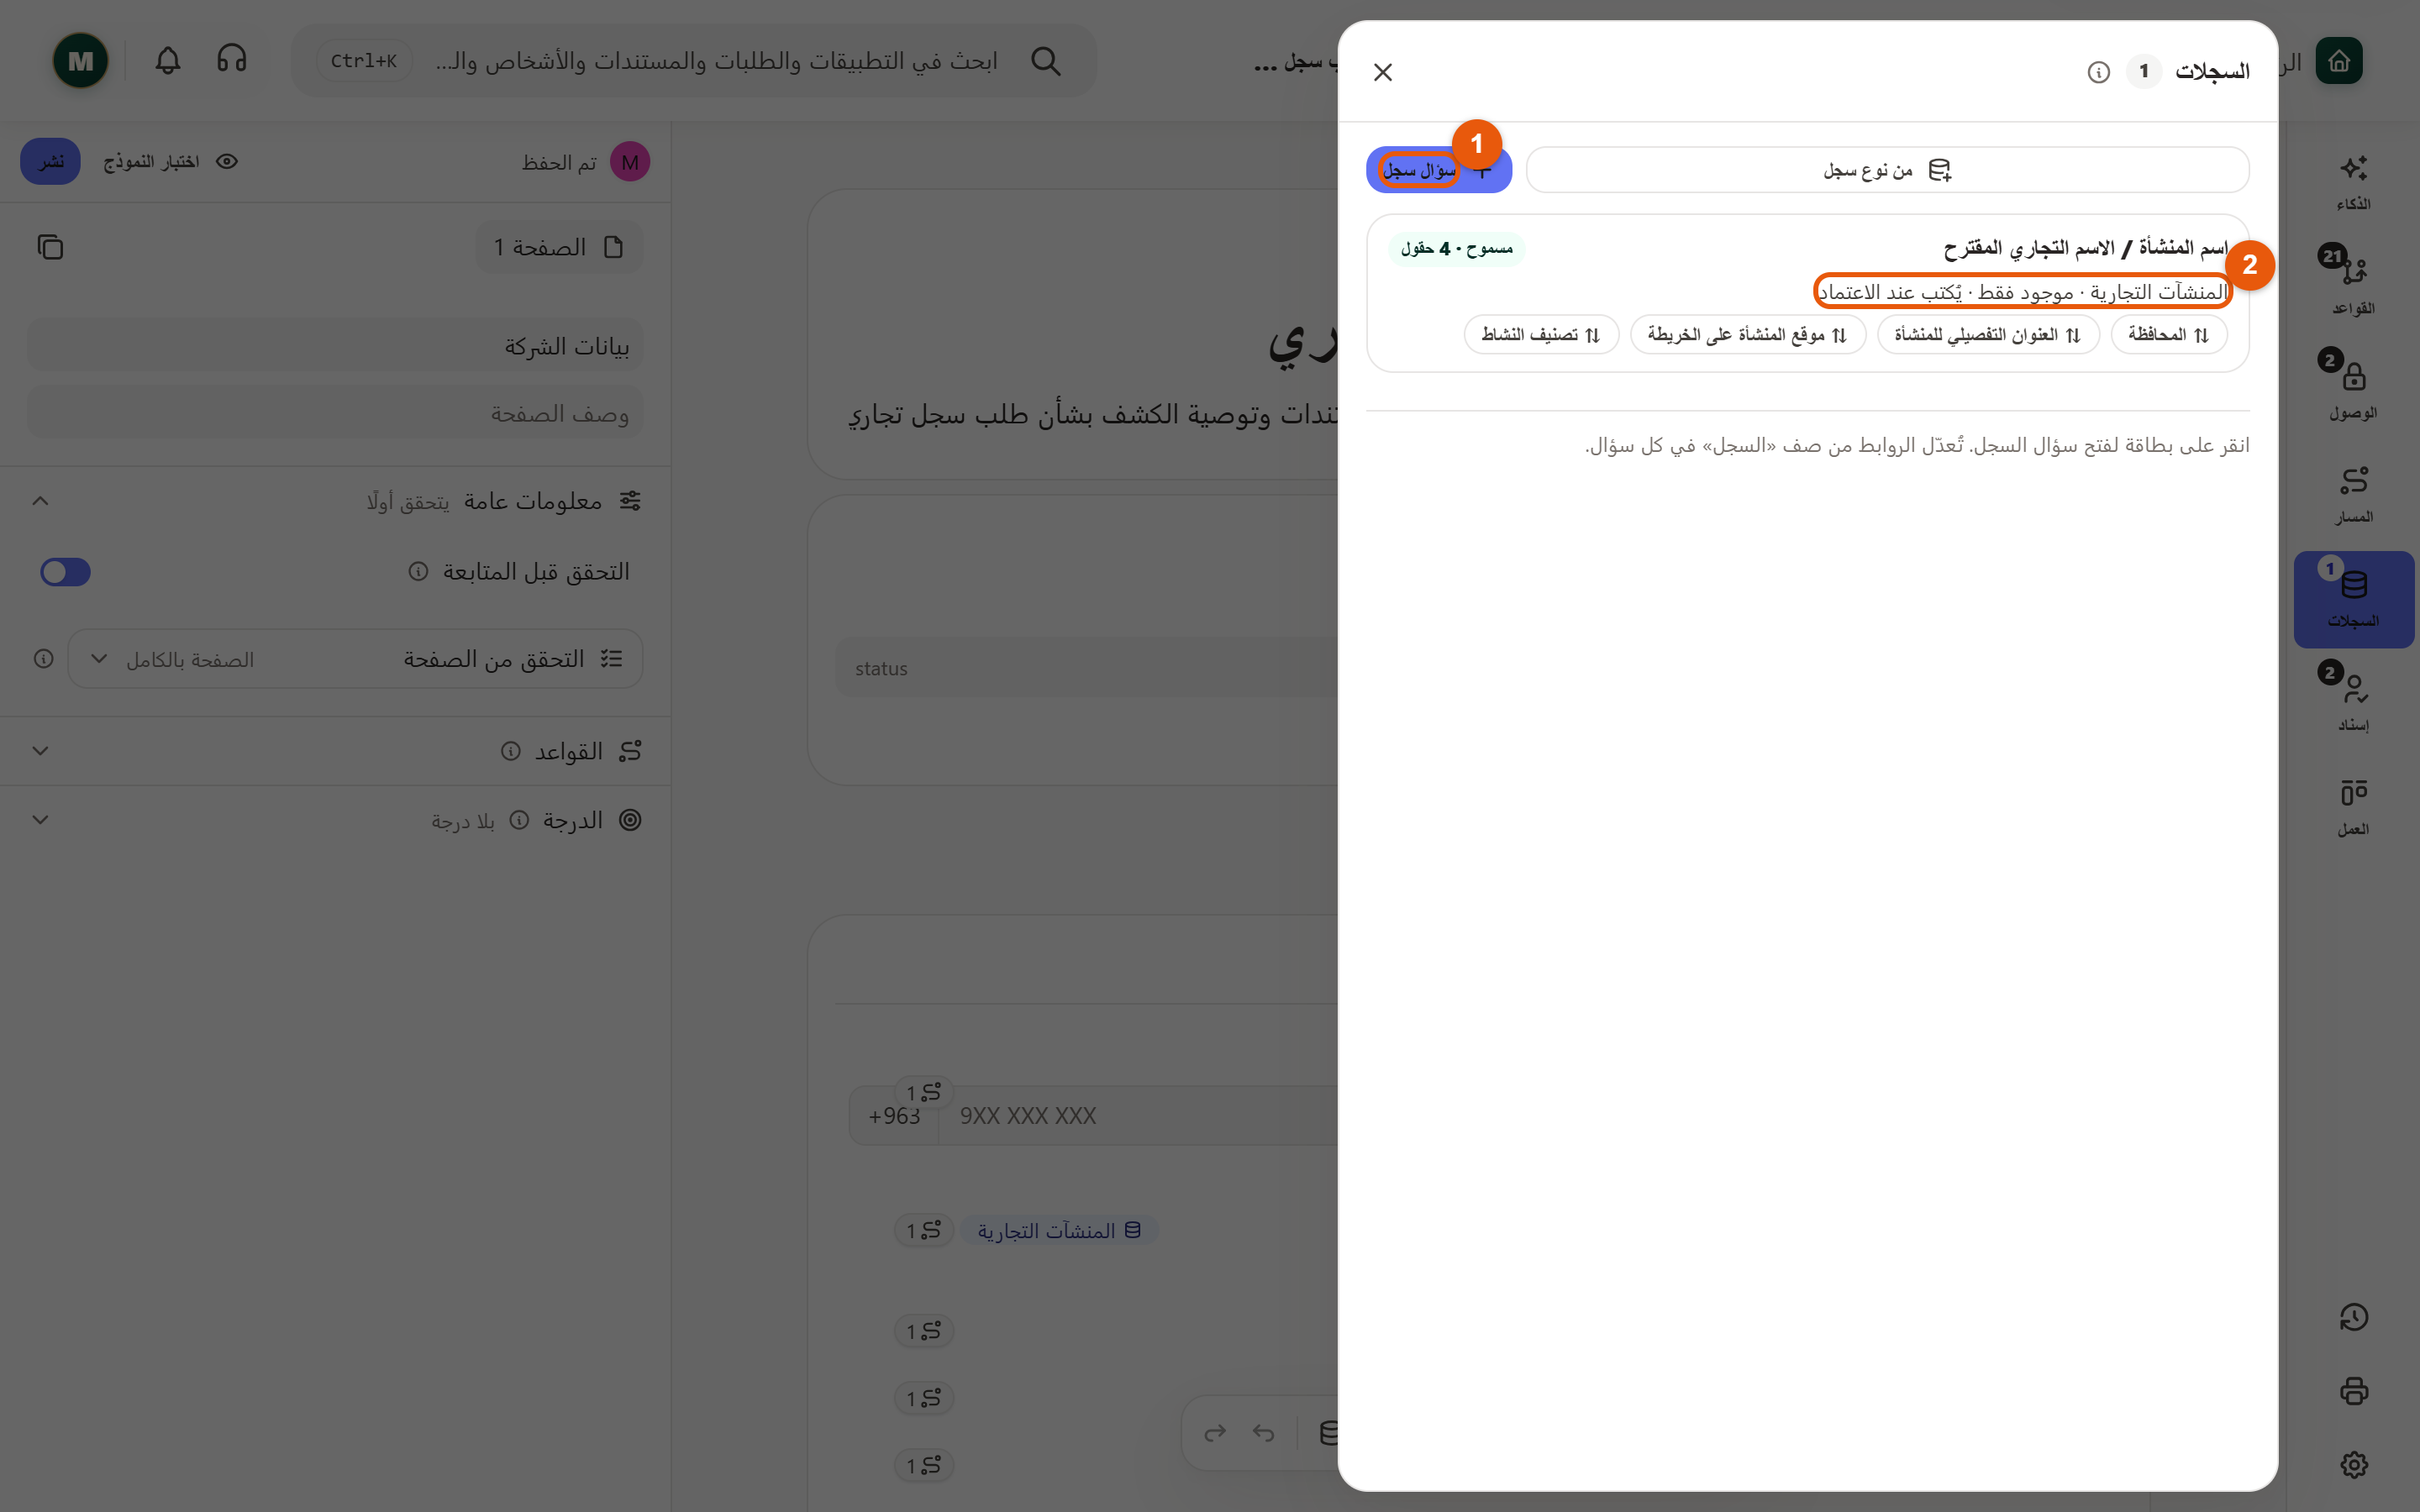
\includegraphics[width=0.95\linewidth]{assets/screens/form-records.png}
\caption{اختيار المنشأة وربط حقولها بالكشف}
\label{fig:record-question}
\shotnote{بطاقة السجل تجمع اختيار المنشأة والحقول المرتبطة بملفها. ① «سؤال سجل»: أضف سؤال اختيار المنشأة. ② ملخص البطاقة: نوع السجل «المنشآت التجارية»، و«موجود فقط» أي يُختار ملف قائم، و«يُكتب عند الاعتماد» أي تنتظر التغييرات المرتبطة الموافقة قبل تحديث ملف المنشأة.}
\end{figure}

\textbf{تحقق:} اضغط «اختبار النموذج»، وافتح سؤال المنشأة. يجب أن تتمكن من اختيار «فرن الأمانة» من القائمة. إذا لم يظهر، تأكد من اختيار نوع «المنشآت التجارية» ومن صلاحية قراءة سجلاته.

\section{اجلب بيانات المنشأة إلى أسئلة الكشف}
\label{sec:build-links}

\textbf{لماذا؟} بعد اختيار الفرن، نريد ظهور عنوانه ومحافظته تلقائياً كي لا يعيد الباحث كتابتهما. وإذا وجد معلومة غير صحيحة في الزيارة، يسجل التصحيح في الكشف.

«سؤال سجل» يختار المنشأة. أما «من نوع سجل» فيضيف أسئلة مأخوذة من حقول تلك المنشأة، مثل المحافظة والعنوان. الأول يحدد \textbf{أي منشأة}، والثاني يحدد \textbf{أي معلومات نأخذ منها}.

\begin{enumerate}
\item افتح «السجلات» داخل النموذج، ثم اضغط «من نوع سجل» بجانب زر «سؤال سجل».
\item اختر «المنشآت التجارية»، ثم اختر سؤال المنشأة الذي أضفته؛ لا تنشئ سؤال اختيار ثانياً.
\item اختر المحافظة، والعنوان التفصيلي، والموقع على الخريطة، والنشاط.
\item للحقول التي تريد أن يصححها الباحث، اختر في عمود «الربط» القراءة والكتابة معاً، وفي عمود «في النموذج» اختر «تعديل». تابع المعالج حتى «مراجعة»، ثم اضغط زر الإضافة الذي يذكر عدد الأسئلة، مثل «إضافة 4 أسئلة».
\item للسماح بعرض معلومة دون تصحيحها، اختر «قراءة فقط» في الربط و«مقفل» في عمود «في النموذج».
\end{enumerate}

\begin{table}[H]
\centering
\caption{كيف تختار نوع الربط؟}
\label{tab:link-modes}
\begin{tabularx}{\linewidth}{R{3cm} Y}
\rcHeaderRow
\thh{الاختيار} & \thh{ما الذي يحدث؟}\\
قراءة & يجلب القيمة المحفوظة من ملف المنشأة إلى الكشف؛ لا يعيد كتابة الملف.\\
كتابة & يرسل إجابة الكشف إلى حقل المنشأة في موعد تطبيق التغييرات.\\
قراءة وكتابة & يجلب القيمة أولاً، ثم يحفظ التصحيح في الملف بعد الاعتماد.\\
مقفل & يرى الباحث الإجابة ولا يستطيع تعديلها. هذا يضبط السؤال نفسه، وليس صلاحية حسابه.\\
\end{tabularx}
\end{table}

\textbf{تحقق:} في «اختبار النموذج»، اختر الفرن. يجب أن يُملأ عنوانه ومحافظته تلقائياً. إذا بقي حقل فارغاً رغم وجود قيمته في الملف، افتح إعداد السؤال وتأكد من الحقل المرتبط ومن تفعيل القراءة.

\subsection{راجع خريطة الربط حقلاً بحقل}

في معالج «من نوع سجل»، اكتب «المنشآت التجارية» في البحث ① واخترها. لأنك أضفت سؤال اختيار المنشأة في الخطوة السابقة، حدده عند ②. الخيار ③ ينشئ سؤال اختيار جديداً، و④ يضيف أسئلة بلا ربط؛ لا تستخدمهما هنا. اضغط ⑤ لتحديد الحقول.

\begin{figure}[H]
\centering
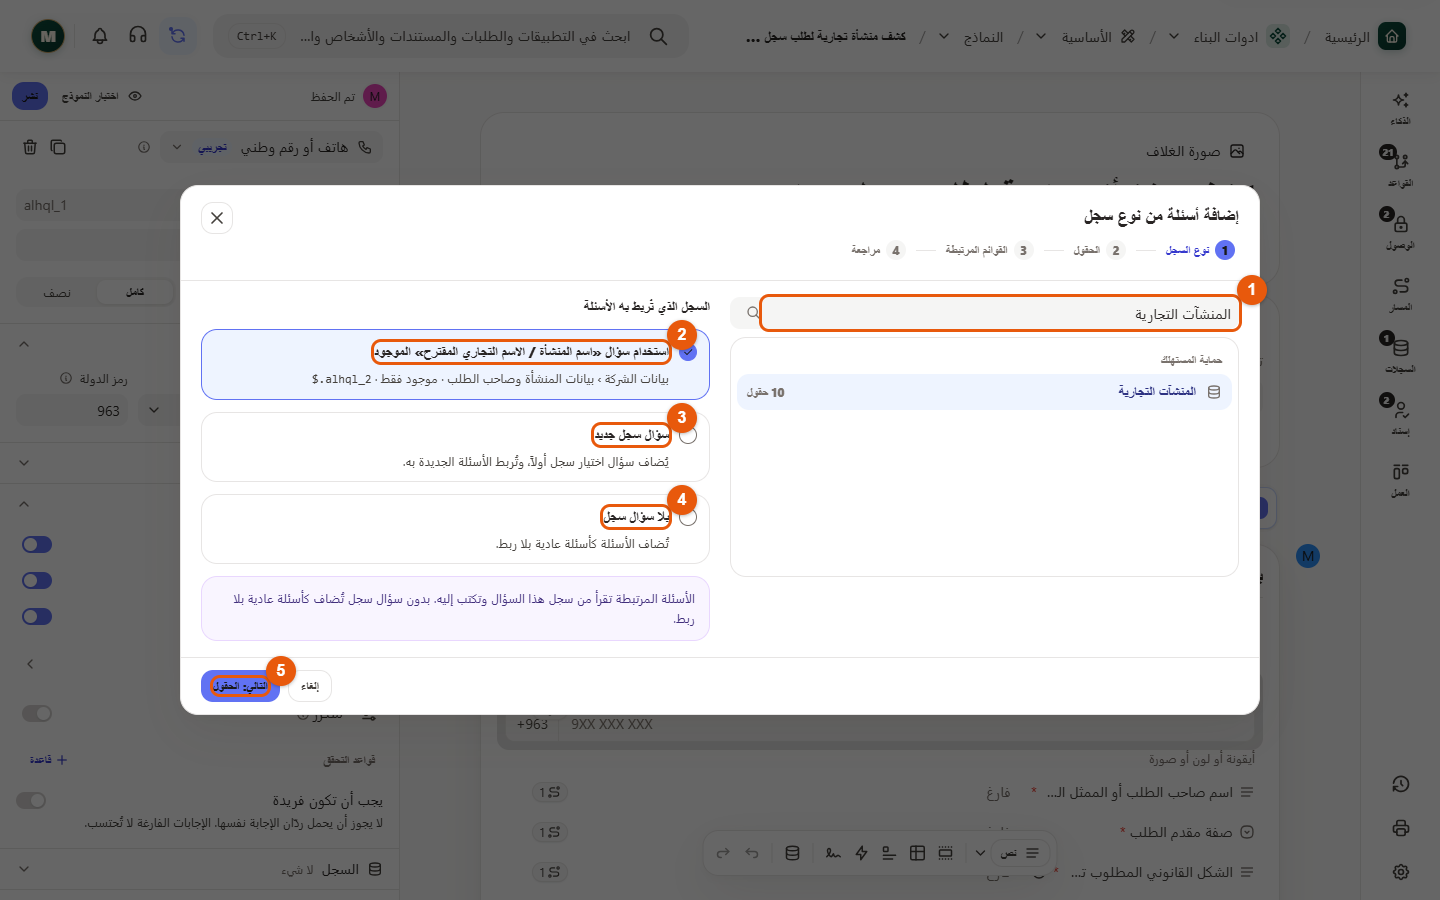
\includegraphics[width=0.95\linewidth]{assets/screens/org-record-source.png}
\caption{تحديد نوع السجلات والسؤال الذي يختار المنشأة}
\label{fig:record-source}
\shotnote{① البحث عن نوع السجلات. ② ربط الحقول بسؤال المنشأة الذي أنشأته. ③ إنشاء سؤال سجل جديد عند الحاجة إلى اختيار مستقل. ④ أسئلة عادية بلا ربط. ⑤ الانتقال إلى اختيار الحقول.}
\end{figure}

في شاشة الحقول، حدد صف الحقل عند ①، واضبط إمكانية تعديله في النموذج عند ②، واتجاه القراءة والكتابة عند ③، ثم راجع التعبئة المسبقة عند ④. بعد إتمام الربط، تميّز العبارة عند ⑤ الحقول المرتبطة بالنموذج. أكمل المعالج من ⑥، وراجع اختياراتك قبل إضافة الأسئلة.

\begin{figure}[H]
\centering
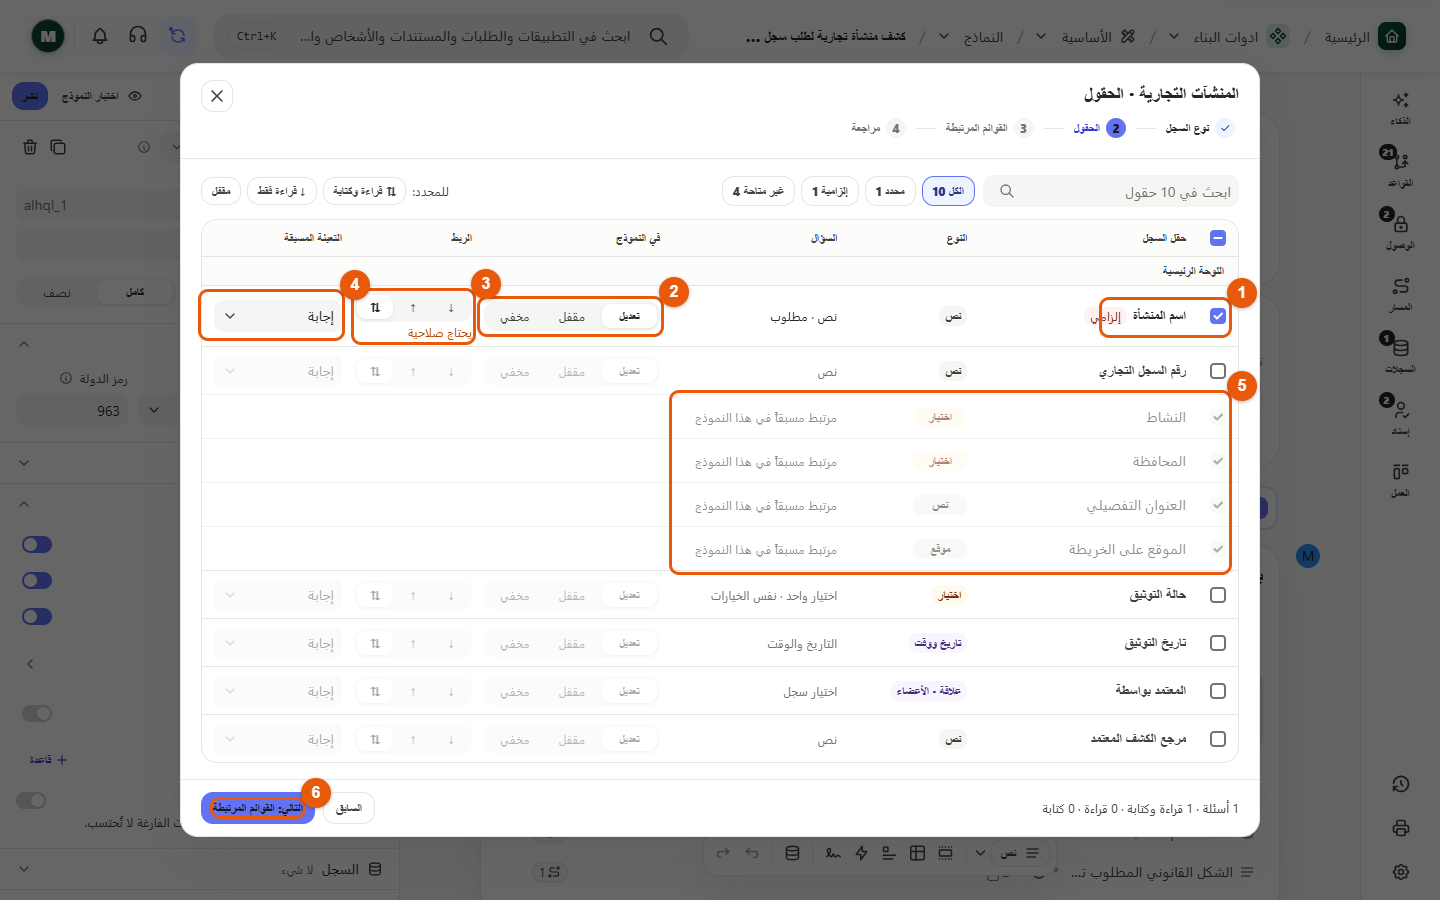
\includegraphics[width=0.95\linewidth]{assets/screens/org-record-fields.png}
\caption{اختيار الحقول واتجاه الربط وطريقة عرض الإجابة}
\label{fig:record-fields}
\shotnote{① تحديد الحقل؛ الاسم المحدد هنا يوضح مكان الاختيار. ② تعديل أو قفل أو إخفاء السؤال. ③ قراءة أو كتابة أو الاثنان، مع تنبيه الصلاحية عند الحاجة. ④ التعبئة المسبقة. ⑤ تظهر الحقول الأربعة بعد ربطها، وليست حقولاً جديدة مختارة للإضافة. ⑥ متابعة المعالج إلى القوائم المرتبطة ثم المراجعة.}
\end{figure}

\begin{table}[H]
\centering
\caption{المصدر والوجهة وموعد التحديث}
\label{tab:field-mapping-detail}
\begin{tabularx}{\linewidth}{R{3cm} Y Y}
\rcHeaderRow
\thh{المعلومة} & \thh{عند اختيار المنشأة} & \thh{بعد الاعتماد}\\
المحافظة & يقرأ السؤال خيار المحافظة من الملف المحدد. & يكتب الخيار الذي صححه الباحث في حقل المحافظة نفسه.\\
العنوان التفصيلي & يعرض عنوان المنشأة في سؤال العنوان. & يحفظ العنوان المصحح في الملف نفسه.\\
الموقع على الخريطة & يجلب الموقع إلى سؤال الموقع. & يحفظ الموقع المصحح إذا سمحت الكتابة له.\\
النشاط & يجلب خيار النشاط بمفتاحه. & يكتب النشاط المعتمد إلى حقل النشاط.\\
الملاحظات والتوصية والمرفقات & تخص زيارة الكشف؛ يملؤها الباحث. & تبقى ضمن الكشف؛ لا تستبدل حقول المنشأة بلا ربط مقصود.\\
\end{tabularx}
\end{table}

افتح إعداد كل سؤال مرتبط، وتأكد من أربعة أشياء: سؤال السجل الذي يحدد المنشأة، وحقل المصدر، واتجاه الربط، وإمكانية تعديل الإجابة. تشابه عنواني سؤالين لا يعني أنهما مربوطان بالحقل نفسه. وكذلك اختيار «كتابة» لا يمنح الإذن للنموذج؛ نضبط الإذن ووقت التطبيق في الخطوة التالية.

\textbf{تحقق:} دوّن عنوان الفرن قبل التجربة، واكتب تصحيحاً في إجابة الكشف. قبل الاعتماد يجب أن يختلف نص الإجابة المصحح عن عنوان الملف القديم؛ وبعد الاعتماد يجب أن يتطابقا. هذه التجربة تثبت القراءة والكتابة وموعد التطبيق معاً.

\section{اجعل التحديث ينتظر اعتماد المدقق}
\label{sec:build-allow}

\textbf{لماذا؟} التصحيح الذي يدخله الباحث يحتاج مراجعة. نريد بقاء العنوان الأصلي في ملف المنشأة حتى تعتمد ريم الكشف، ثم انتقال التصحيح إلى الملف.

\begin{enumerate}
\item افتح «السجلات» داخل النموذج، ثم بطاقة المنشأة، واضبط تطبيق الكتابة على «عند الاعتماد».
\item عند ظهور طلب السماح، اضغط «السماح في نوع السجل». هذا إذن للنموذج بأن يغيّر حقولاً محددة في ملف المنشأة.
\item راجع الحقول المطلوبة للكتابة: المحافظة والعنوان والموقع والنشاط، ثم اضغط «موافقة».
\item تأكد من ظهور «مسموح · 4 حقول» في بطاقة الربط. لا تمنح الكتابة لأسئلة الملاحظات أو المرفقات إذا كانت تخص الزيارة فقط.
\end{enumerate}

\textbf{تحقق:} تظهر عبارة «يُكتب عند الاعتماد» كما في صورة سؤال السجل. إذا بقي الطلب «بانتظار موافقة مسؤول»، فلن يطبق النموذج تحديثاته حتى يوافق مسؤول نوع السجلات.

\section{حدّد كيف ينتقل الكشف إلى المدقق}
\label{sec:build-journey}

\textbf{لماذا؟} «الحالة» تخبرنا أين وصل الكشف: مسودة، أو قيد التدقيق، أو مقبول. «خطوة الموافقة» تحدد الشخص الذي يقرر. و«الانتقال» ينقل الكشف من حالة إلى أخرى عند الإرسال أو القرار.

\begin{enumerate}
\item افتح «المسار» في النموذج، واضغط «تفعيل المسار» ثم «تفعيل خطوات الموافقة» إن لم يكونا مفعّلين.
\item استخدم حالة «قيد التدقيق» لعمل المدقق. اضبط انتقال الإرسال ليصل الكشف إليها بعد أن يرسله الباحث؛ يمكن أن يمر بحالة «مُرسل» أولاً.
\item اضغط «خطوة موافقة»، واكتب «تدقيق كشف المنشأة». في «تعمل في» اختر «قيد التدقيق»، وفي «تبدأ» اختر «عند الوصول إلى حالتها».
\item في «من يوقّع»، افتح «المعتمِد» ← «محدد العضوية»، واختر منصب «مدقق كشوف المنشآت — 01». بهذا تصل الموافقة إلى ريم، شاغلة المنصب.
\item اضبط نتائج الخطوة وفق الجدول. ثم افتح «الفحص» وأصلح أي تحذير بأن الموقّع غير محدد أو أن انتقالاً يتجاوز خطوة الموافقة.
\end{enumerate}

\begin{table}[H]
\centering
\caption{قرارات المدقق وما يحدث بعدها}
\label{tab:decisions}
\begin{tabularx}{\linewidth}{R{3cm} R{3cm} Y}
\rcHeaderRow
\thh{الزر} & \thh{الحالة التالية} & \thh{المعنى}\\
اعتماد الكشف & مقبول & انتهى التدقيق بالموافقة، وتُطبق الكتابة المسموح بها.\\
رفض & مرفوض & انتهى الكشف دون اعتماد التصحيح؛ اجعل التعليق مطلوباً لتوضيح السبب.\\
إعادة للتصحيح & بحاجة إلى تصحيح & يعود للباحث ليستكمل البيانات؛ اجعل التعليق مطلوباً.\\
\end{tabularx}
\end{table}

\begin{figure}[H]
\centering
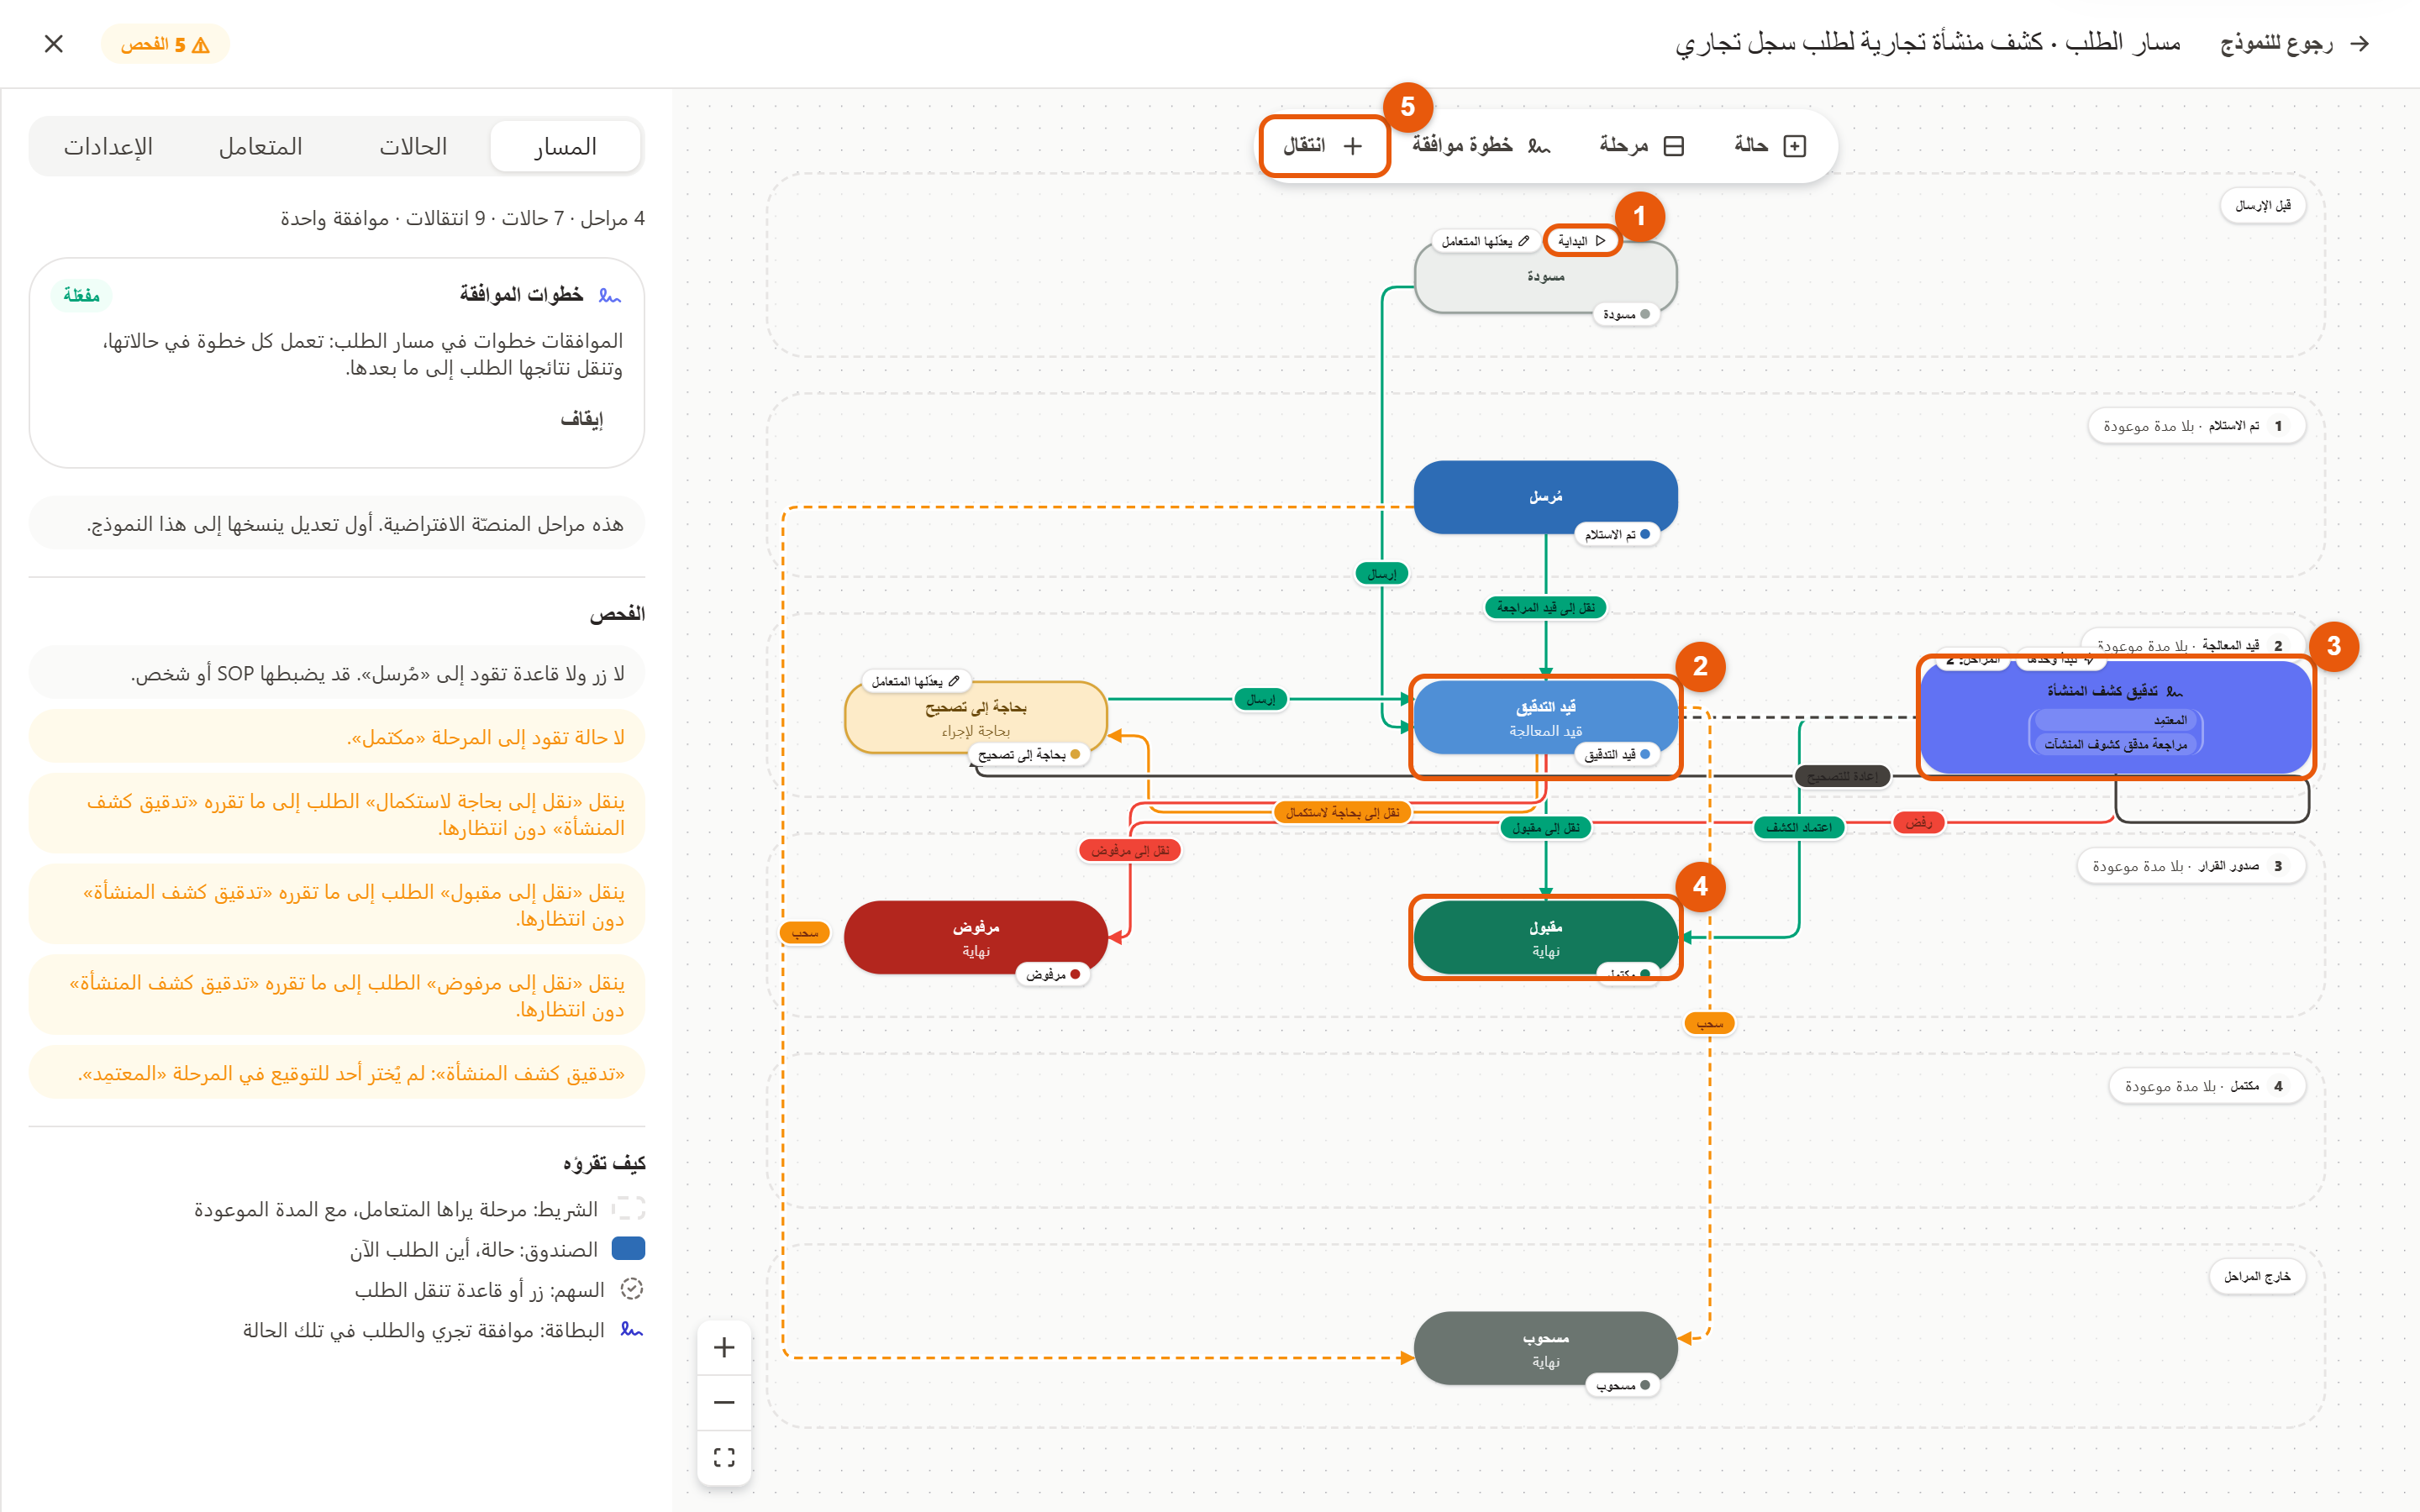
\includegraphics[width=0.95\linewidth]{assets/screens/journey-map.png}
\caption{إعداد مسار الكشف وخطوة الموافقة}
\label{fig:journey}
\shotnote{توضح الخريطة الفرق بين الحالات وخطوة القرار، وتظهر فيها ملاحظات الفحص التي يجب معالجتها قبل النشر. ① البداية. ② حالة «قيد التدقيق». ③ خطوة «تدقيق كشف المنشأة». ④ حالة «مقبول». ⑤ أداة إضافة انتقال.}
\end{figure}

\textbf{تحقق:} لا يصل الكشف إلى «مقبول» إلا من نتيجة اعتماد المدقق. وعند الإعادة، يستطيع الباحث تعديل الإجابة ثم إرسالها إلى التدقيق مجدداً.

\subsection{اضبط كل قرار ووجهته، وليس اسم الزر فقط}

\begin{enumerate}
\item افتح خطوة «تدقيق كشف المنشأة» وراجع حالتها «قيد التدقيق» ومتى تبدأ. وجود الحالة على الخريطة وحده لا ينشئ تكليف الموافقة؛ يجب أن تعمل الخطوة عند الوصول إليها.
\item راجع الموقّع: اختر المنصب «مدقق كشوف المنشآت — 01»، ثم تأكد أن ريم تشغله بتعيين نشط. اختيار منصب صحيح بلا شاغل لا يحدد شخصاً يستطيع اتخاذ القرار.
\item افتح إعداد نتيجة «اعتماد الكشف»، واربطها بالموافقة والحالة «مقبول». اسم الزر وصف يراه المدقق؛ أثره يأتي من النتيجة والانتقال المضبوطين له.
\item افتح نتيجة «رفض»، واربطها بالرفض والحالة «مرفوض»، واطلب تعليقاً يشرح السبب. لا تربط الرفض بحالة القبول لمجرد إنهاء الطلب.
\item افتح نتيجة «إعادة للتصحيح»، واربطها بالحالة «بحاجة إلى تصحيح»، واطلب توضيح المطلوب. راجع إمكانية تعديل الباحث ثم انتقال إعادة الإرسال إلى «قيد التدقيق».
\item إذا فعّلت اشتراط قراءة الأقسام أو إقرار المدقق، اكتب المطلوب بوضوح وجربه بحساب المدقق. هذه شروط لاتخاذ القرار؛ ليست بديلاً عن تحديد الموقّع.
\item افتح «الفحص»، وراجع تحذيرات الحالات والانتقالات والتوقيع. تتبع المسار من البداية بإصبعك: إرسال، ثم تدقيق، ثم واحدة من النتائج الثلاث. لا تترك طريقاً آخر يقبل الكشف قبل قرار ريم.
\end{enumerate}

افتح «الفحص» وطابق التنبيهات مع الأرقام في الصورة التالية. عالج ① بتحديد الموقّع في خطوة الموافقة، ثم ② بمراجعة انتقال القبول كي ينتظر نتيجتها، ثم ③ بربط المرحلة بالحالة التي تشغّلها. أعد الفحص بعد كل تصحيح؛ اختفاء تنبيه لا يعني أن بقية المسار اكتملت.

\begin{figure}[H]
\centering
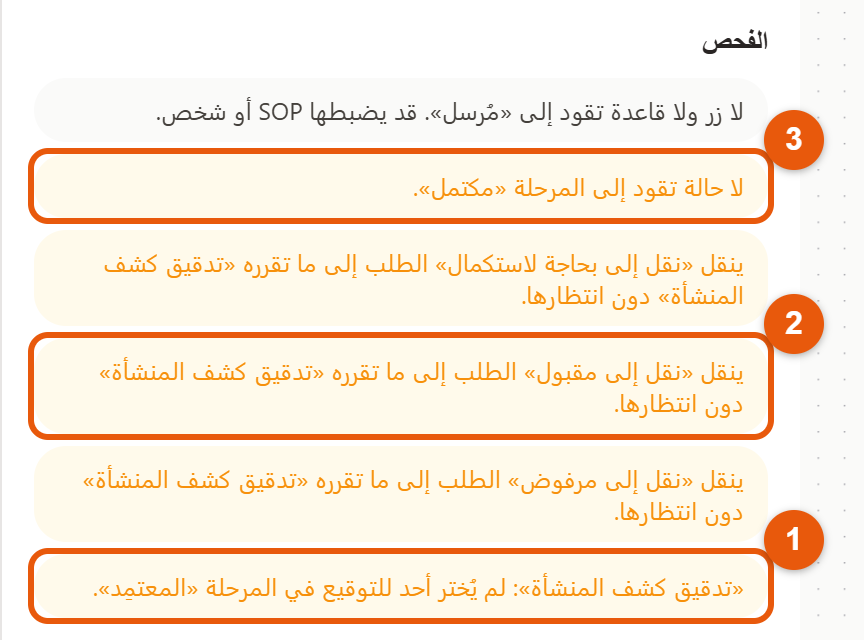
\includegraphics[width=0.8\linewidth]{assets/screens/journey-check.png}
\caption{قراءة تنبيهات فحص المسار وإصلاح أسبابها}
\label{fig:journey-check}
\shotnote{هذه شاشة تشخيص قبل اكتمال إعداد المسار. ① لم يُختر أحد للتوقيع: افتح المعتمِد وحدد منصب المدقق. ② انتقال إلى مقبول دون انتظار الموافقة: راجع شرط الانتقال ونتيجة خطوة التدقيق. ③ لا حالة تقود إلى المرحلة: راجع ربط المرحلة بالحالة؛ لا تترك مرحلة لا يمكن الوصول إليها.}
\end{figure}

\textbf{تحقق:} تستطيع الإجابة عن أربعة أسئلة لكل سهم: ما الذي يشغله؟ من يملك تنفيذه؟ إلى أين يصل؟ وهل يطبق كتابة على المنشأة؟ لا تنشر مساراً تعرف أسماء حالاته ولا تعرف ما ينقل الإجابة بينها.

\section{امنح الوصول وانشر النموذج}
\label{sec:build-publish}

\textbf{لماذا؟} معرفة النظام بمنصب نور لا تمنحه كل الصلاحيات تلقائياً. نحدد ما يسمح له بفعله، ثم ننشر نسخة جاهزة للفريق. الحفظ يحتفظ بإعداداتك، أما النشر فيجعل النسخة الجديدة متاحة للعمل.

\begin{enumerate}
\item في النموذج، افتح «الوصول» ← «إضافة» بجانب «أشخاص ثابتون».
\item اختر منصب «باحث ميداني — 01»، وامنحه «قائمة» و«فتح» و«إرسال الطلبات»، ثم اضغط «حفظ في المسودة».
\item أضف منصب «مدقق كشوف المنشآت — 01» ومنصب رئيس الفريق مع «قائمة» و«فتح». قرار التدقيق يصل إلى المدقق من خطوة الموافقة التي أعددتها.
\item افتح «الإعدادات» ← «الأدوار» ← «إضافة الدور». اكتب «مراقب حماية المستهلك» في «عنوان الدور»، وأدخل الكود \en{mraqb\_hmayt\_almsthlk}، ثم اضغط «إنشاء الدور». الدور مجموعة صلاحيات يمكن منحها لعدة مناصب.
\item في صفحة الدور، افتح «المسؤولين» ← «تعيين الأعضاء والمناصب والعقد»، واختر مناصب الباحث والمدقق ورئيس الفريق التي أنشأناها.
\item افتح «المنشآت التجارية» ← «الصلاحيات» ← «الأدوار». في صف «مراقب حماية المستهلك»، فعّل «قائمة» و«فتح»، ثم «المراجعة والنشر» ← «نشر». «قائمة» تُظهر السجلات، و«فتح» يسمح بقراءة ملف المنشأة.
\item عد إلى النموذج واضغط «اختبار النموذج». اختر منشأة، وتأكد من ظهور بياناتها والأسئلة المطلوبة.
\item اضغط «نشر»، واقرأ ملخص التعديلات، ثم أكّد النشر.
\end{enumerate}

\begin{figure}[H]
\centering
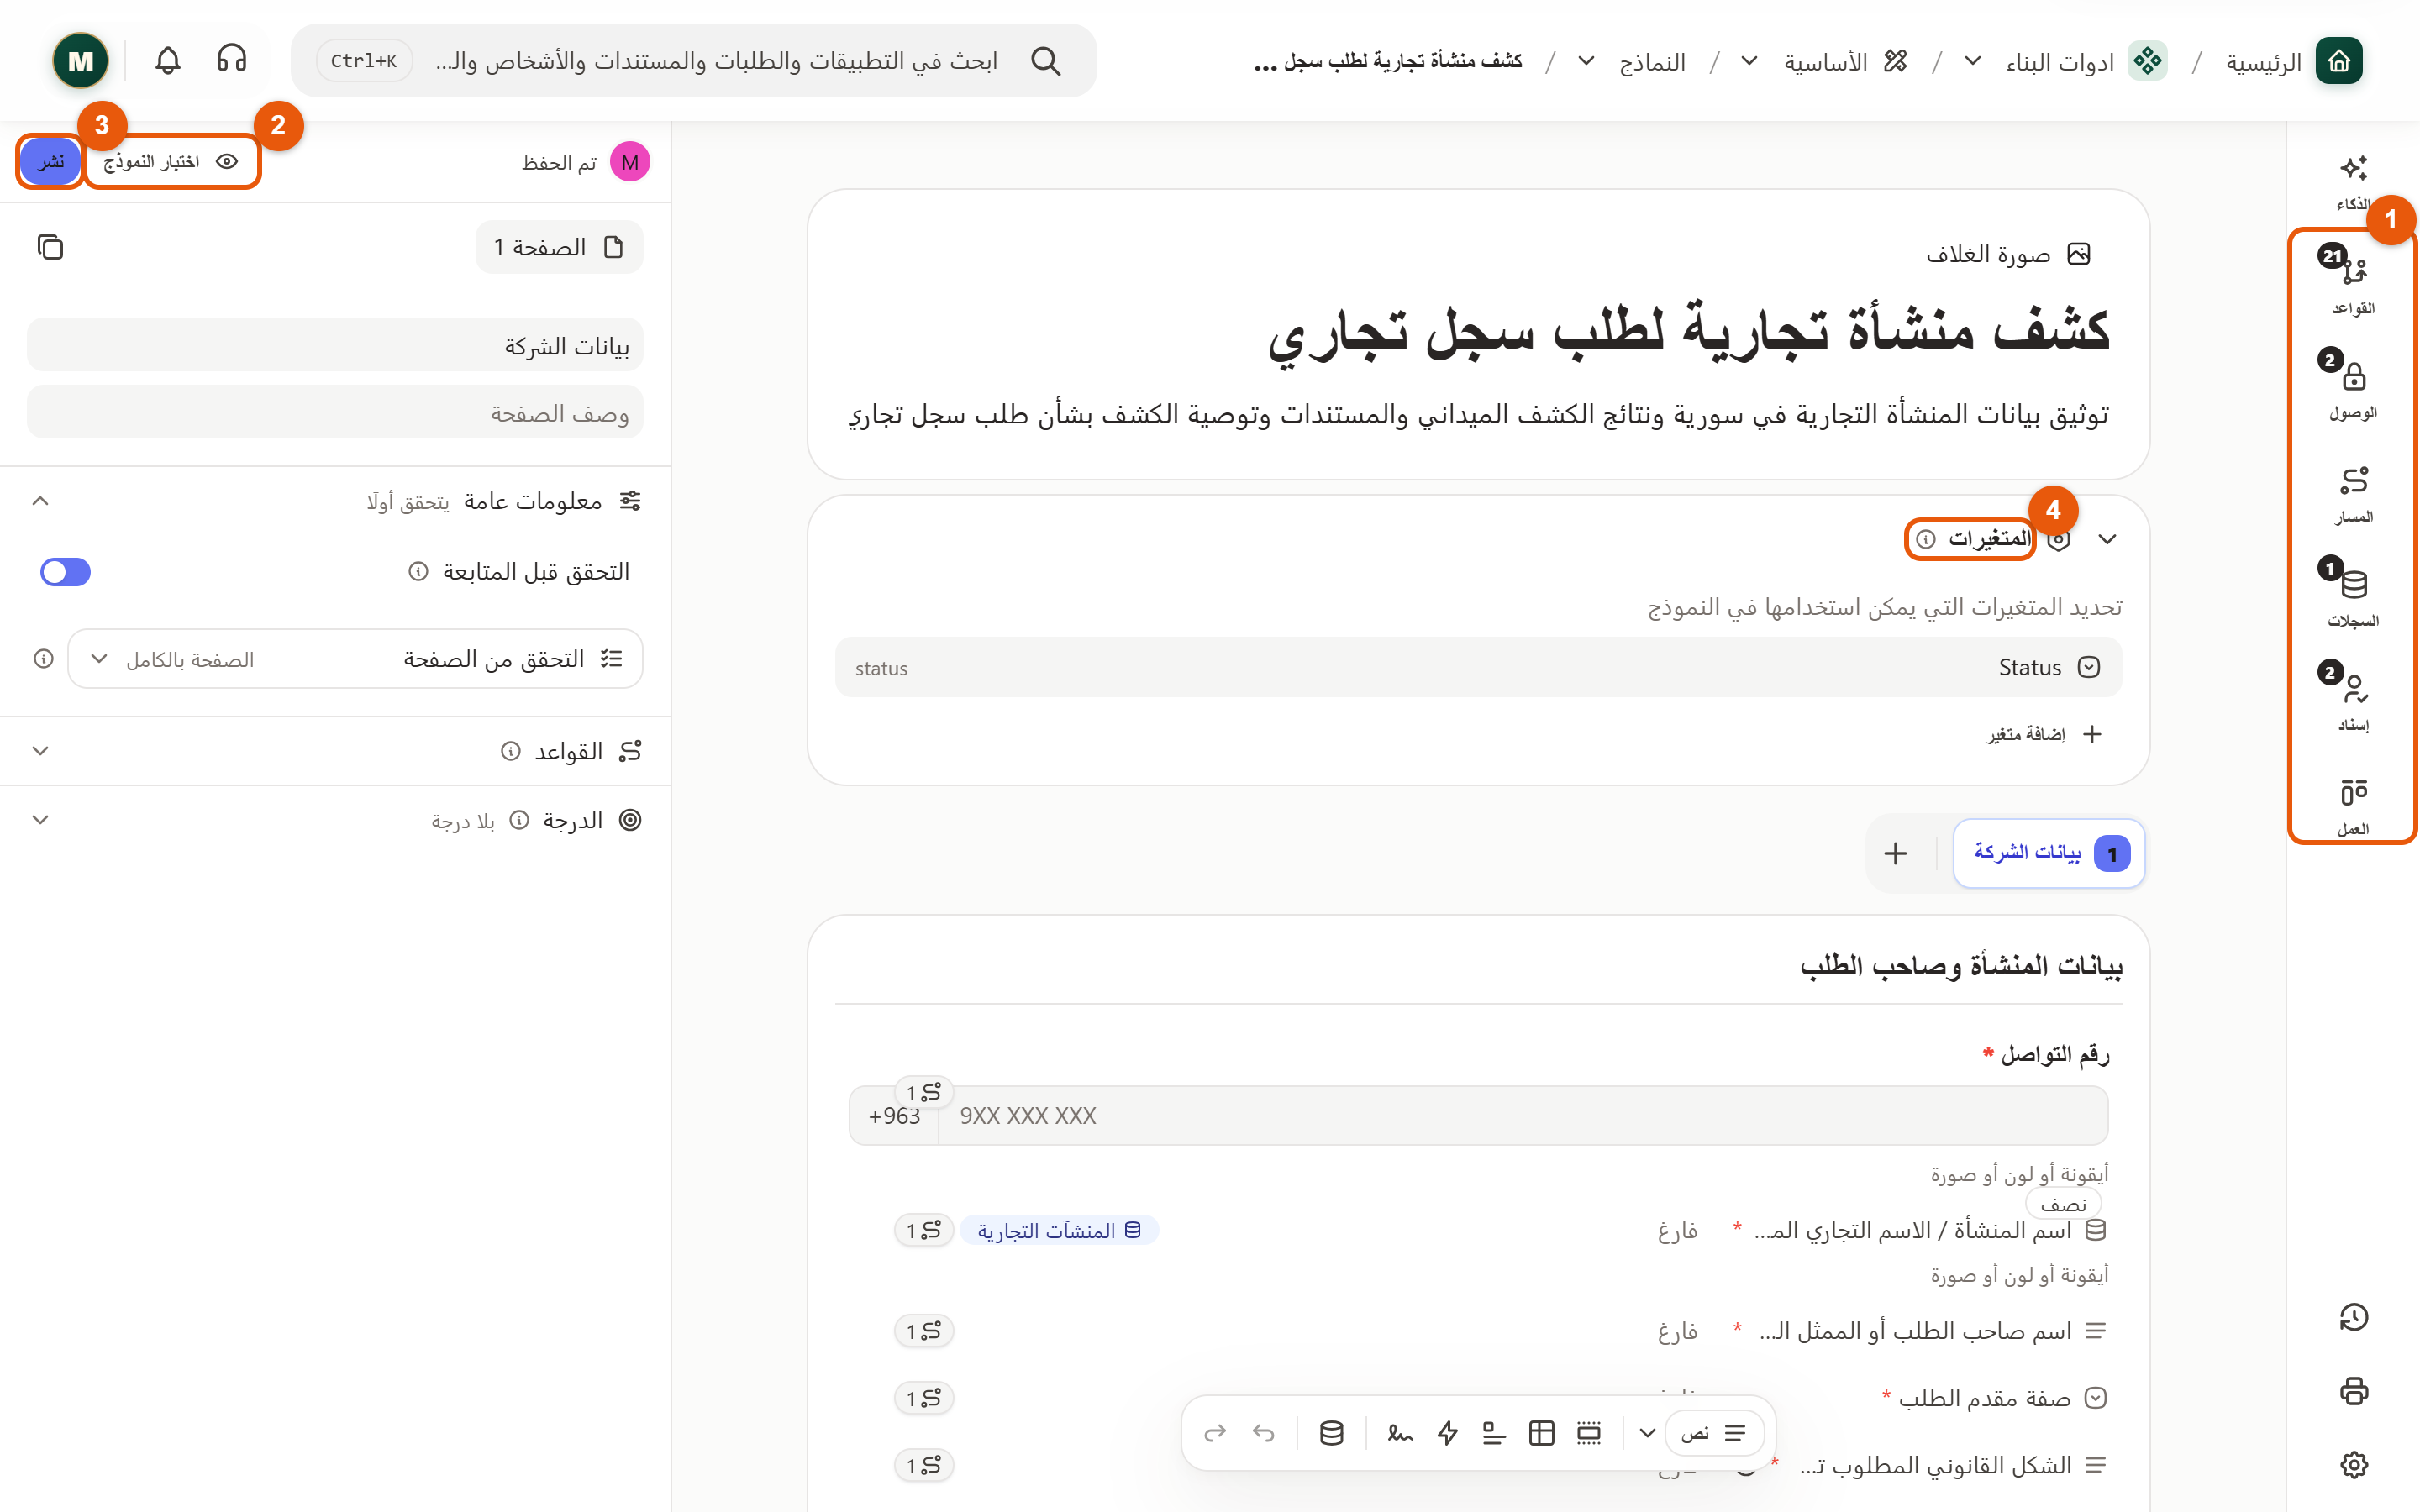
\includegraphics[width=0.95\linewidth]{assets/screens/form-builder.png}
\caption{أدوات الإعداد والاختبار والنشر}
\label{fig:builder}
\shotnote{الشريط الجانبي يجمع الإعدادات التي أكملتها، بينما يبقى الاختبار والنشر أعلى المحرر. ① أدوات الربط والوصول والمسار والتكليف. ② «اختبار النموذج»: جرّب الأسئلة قبل التشغيل. ③ «نشر»: أتح النسخة للفريق. ④ «المتغيرات»: قيم يستخدمها النموذج، ولا تحتاج لإضافة متغير جديد لمجرد ربط المنشأة.}
\end{figure}

\textbf{تحقق:} يستطيع الباحث فتح النموذج وقراءة المنشأة. إذا ظهر منع وصول، افحص صلاحية النموذج وصلاحية «المنشآت التجارية» كلّاً على حدة.

\subsection{افصل الصلاحيات حتى تعرف سبب كل منع}

الوصول إلى النموذج يسمح لنور بتعبئة الكشف. قراءة المنشآت تسمح له باختيار الفرن ورؤية بياناته. إذن كتابة النموذج يسمح بتطبيق الحقول المحددة بعد الاعتماد. وإسناد خطوة الموافقة يجعل ريم صاحبة القرار. هذه أربعة إعدادات مختلفة؛ منح أحدها لا يعوض غياب الآخر، ولا يحتاج الباحث إلى صلاحيات إدارة أدوات البناء لينفذ زيارة.

\subsection{اختبر النسخة قبل تكليف الفريق}

\begin{table}[H]
\centering
\caption{اختبارات النموذج ونتائجها المطلوبة}
\label{tab:form-acceptance}
\begin{tabularx}{\linewidth}{Y Y}
\rcHeaderRow
\thh{التجربة} & \thh{النتيجة التي تبحث عنها}\\
الإرسال دون منشأة أو توصية & يظهر تنبيه واضح ويمنع الإرسال الناقص.\\
اختيار الفرن & تمتلئ الحقول المرتبطة من ملفه.\\
التوصية بعدم الموافقة دون أسباب & تعمل قاعدة الإلزام، ثم تزول المشكلة بعد كتابة السبب.\\
تصحيح العنوان ثم إرسال الكشف & يبقى عنوان الملف القديم إلى حين اعتماد التغيير.\\
إعادة الكشف من ريم إلى نور & يصل السبب لنور ويستطيع التصحيح وإعادة الإرسال.\\
رفض كشف & لا يعتمد التصحيح ولا يكتب إلى الملف.\\
اعتماد كشف & يصبح مقبولاً وتظهر نتيجة تطبيق تحديثات المنشأة.\\
فتح النموذج بحساب الباحث & تعمل صلاحياته دون الاعتماد على صلاحيات المسؤول الذي بناه.\\
\end{tabularx}
\end{table}

استخدم «اختبار النموذج» للأسئلة والقواعد والقراءة. أما وصول التكليف والتدقيق وتطبيق الكتابة فاختبرها عبر كشف فعلي وفق الخطوات التالية؛ المعاينة وحدها لا تثبت دورة العمل. اختبر الرفض والاعتماد بكشفين منفصلين، وسجل النتيجة المتوقعة قبل كل تجربة. بعد أي تعديل مؤثر، انشر النسخة واختبر إجابة جديدة عليها.

\textbf{تحقق:} لا تعتبر النموذج جاهزاً لمجرد أن نشره نجح. الجاهزية تعني أن الباحث يستطيع تعبئته، والمدقق يستطيع اتخاذ القرارات الثلاثة، وأن الكتابة تحدث في الموعد المحدد وعلى الملف الصحيح.

\section{كلّف الباحث بالكشف على المنشأة}
\label{sec:build-plan}

\textbf{لماذا؟} النموذج يحدد ما سيملؤه الباحث. أما «خطة التكليف» فتحدد من سيملؤه، وعن أي منشأة، ومتى. سنطلب من نور تعبئة نموذج الكشف عن فرن الأمانة.

\begin{enumerate}
\item افتح النموذج ← «إسناد»، وفعّل «يمكن التكليف به».
\item اختر «تعبئة وإرسال» في صلاحيات المكلّف. وفي «سؤال السجل» اختر سؤال «اسم المنشأة / الاسم التجاري المقترح»؛ هكذا يفتح التكليف والفرن محدد مسبقاً.
\item في «ينتهي التكليف عندما تصبح الإجابة» اختر «مقبولة» إذا أردت أن تبقى المهمة مفتوحة حتى اعتماد المدقق؛ أما «مُرسلة» فتنهيها بمجرد الإرسال. ثم انشر التعديل.
\item افتح «خطط التكليف» ← «خطة جديدة». اختر نموذج «كشف منشأة تجارية لطلب سجل تجاري»، واكتب اسماً يصف الجولة، ثم اضغط «إنشاء والإعداد».
\item في خطوة «السجلات» حدد «المنشآت التجارية» والمنشأة «فرن الأمانة». وفي خطوة «المرشحون» اختر «قائمة ثابتة» في «المرشحون من»، وأضف «باحث ميداني — 01».
\item اضغط «تشغيل المعاينة». يجب أن تقابل «فرن الأمانة» العضو «نور حسن — تجريبي». حدد الموعد المطلوب، ثم اضغط «حفظ» و«إنشاء التكليفات».
\end{enumerate}

\begin{figure}[H]
\centering
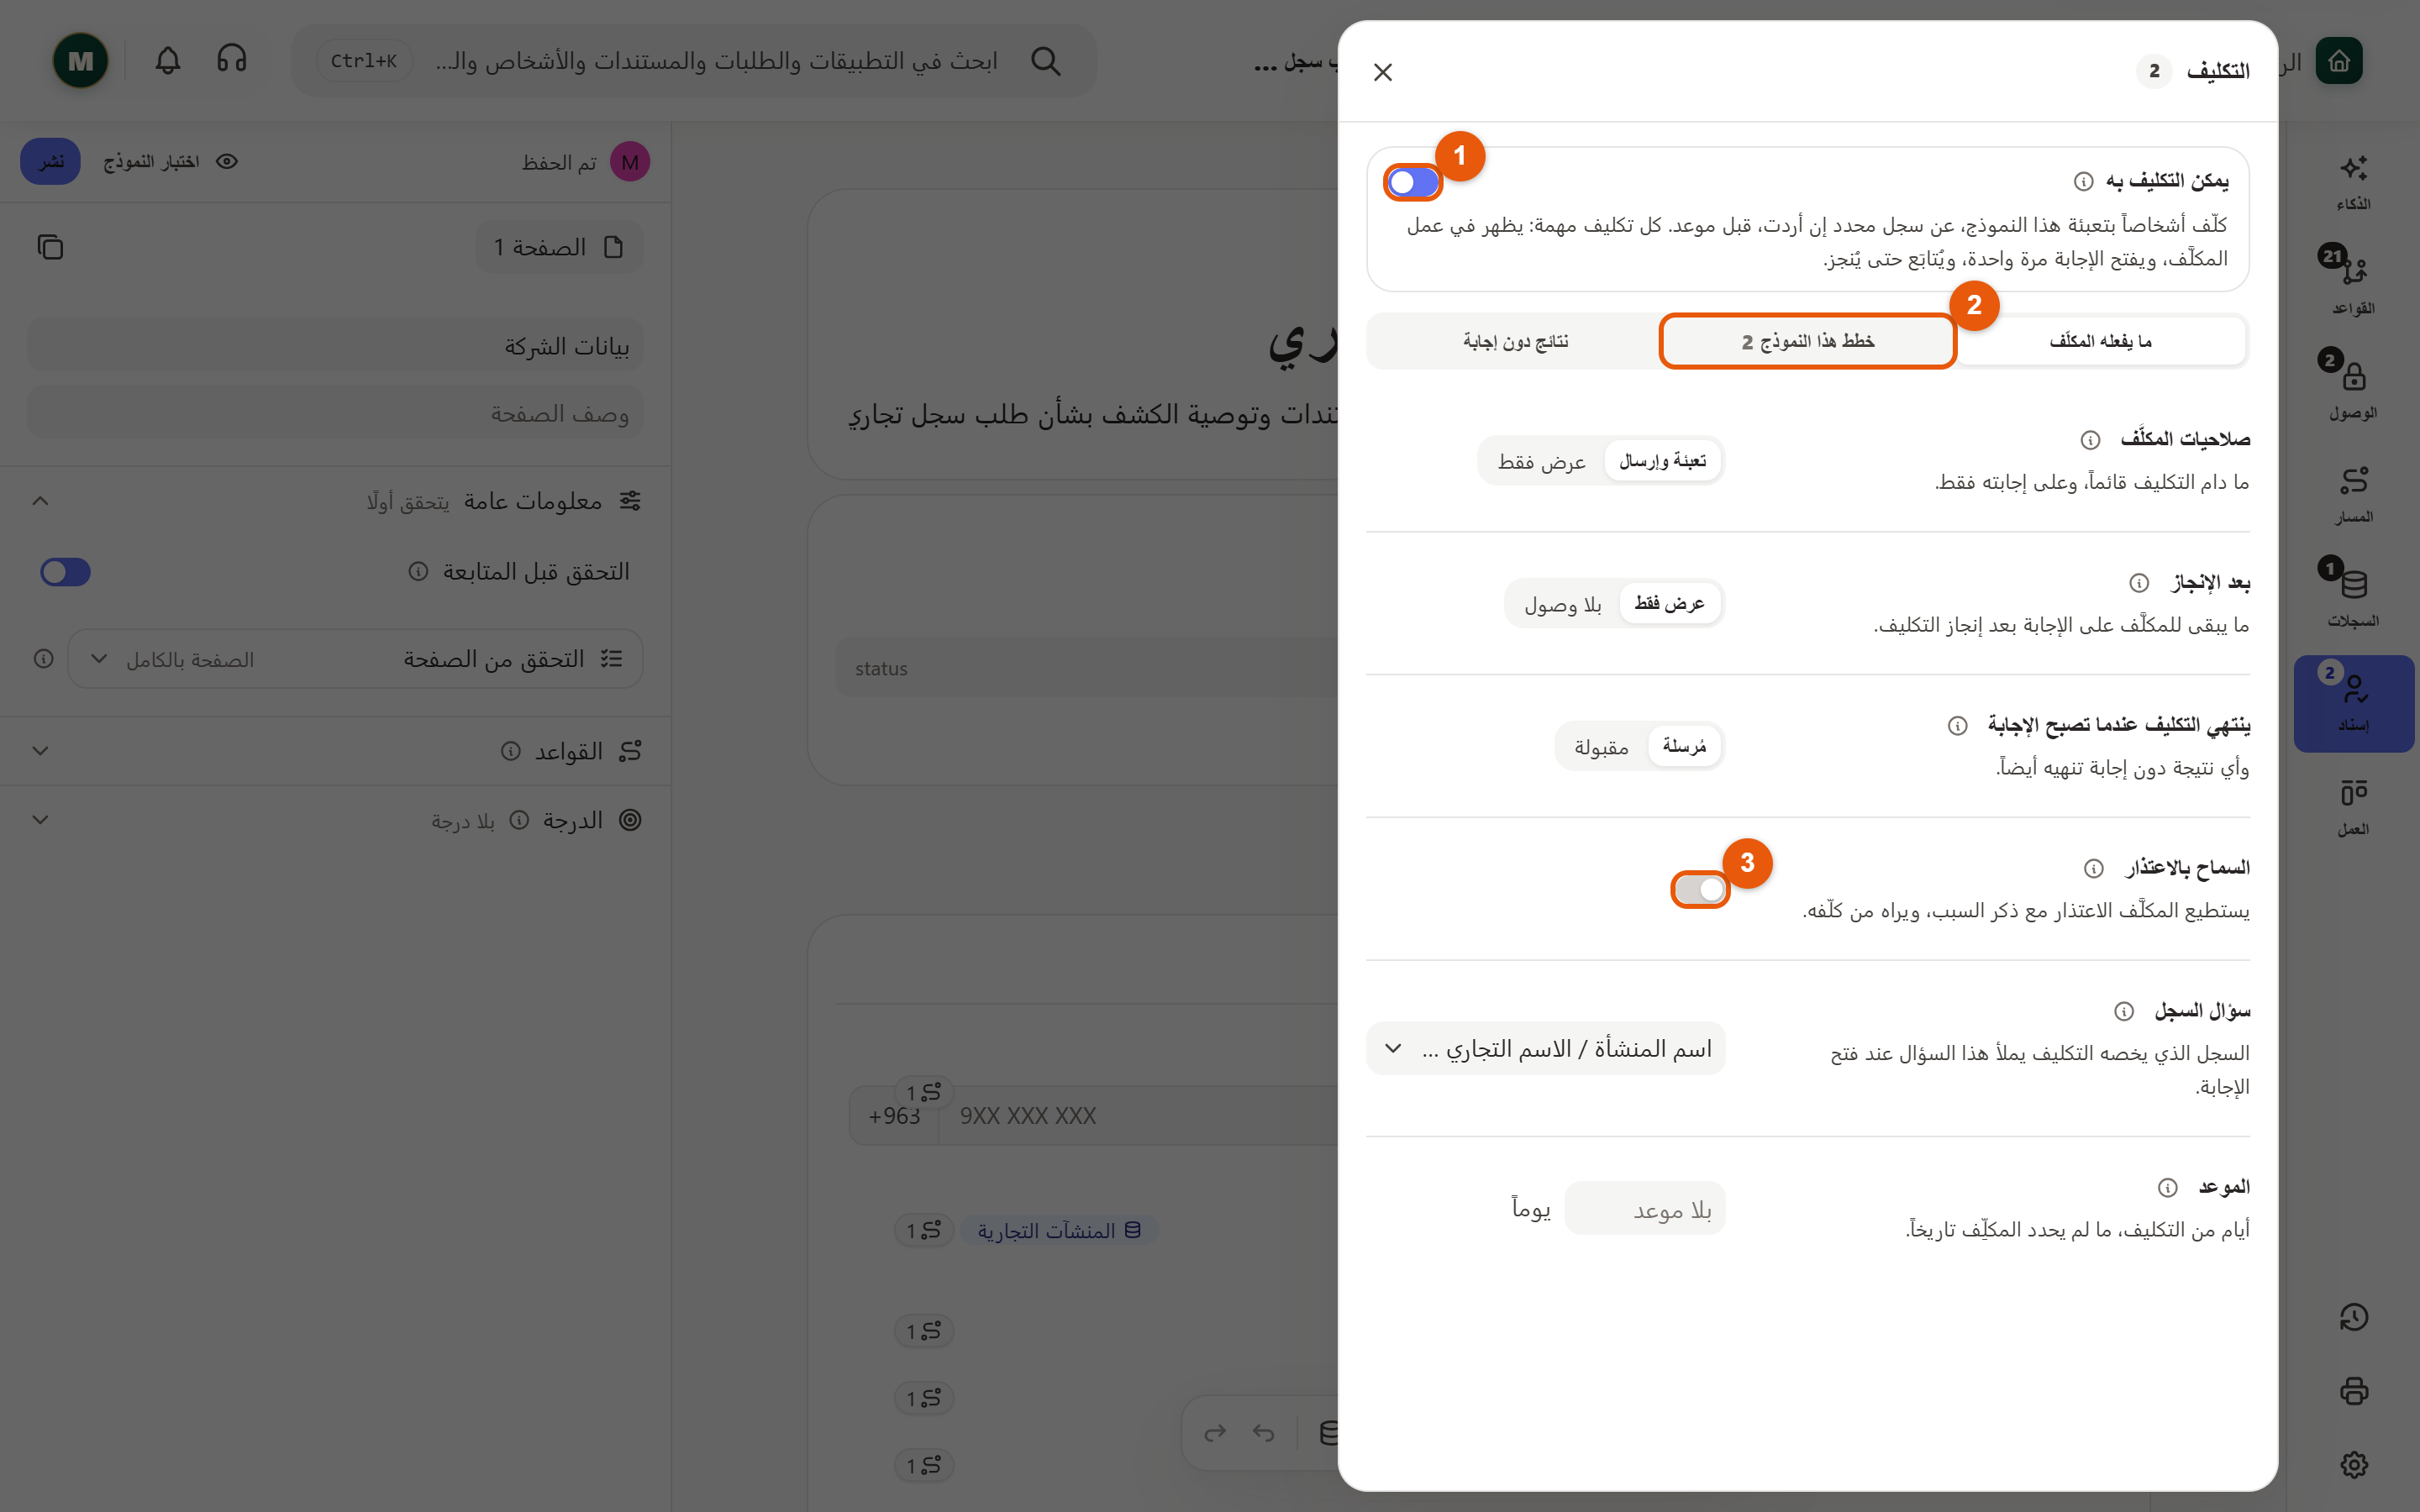
\includegraphics[width=0.95\linewidth]{assets/screens/form-assign.png}
\caption{السماح بتكليف شخص بتعبئة النموذج}
\label{fig:assign}
\shotnote{تحدد هذه الشاشة كيف يعمل التكليف، وما يمكن للباحث فعله في إجابته. ① «يمكن التكليف به»: فعّل استخدام النموذج في الخطط. ② «خطط هذا النموذج»: افتح الخطط المرتبطة به. ③ «السماح بالاعتذار»: خيار إضافي إن كانت إجراءات العمل تسمح باعتذار الباحث.}
\end{figure}

\begin{figure}[H]
\centering
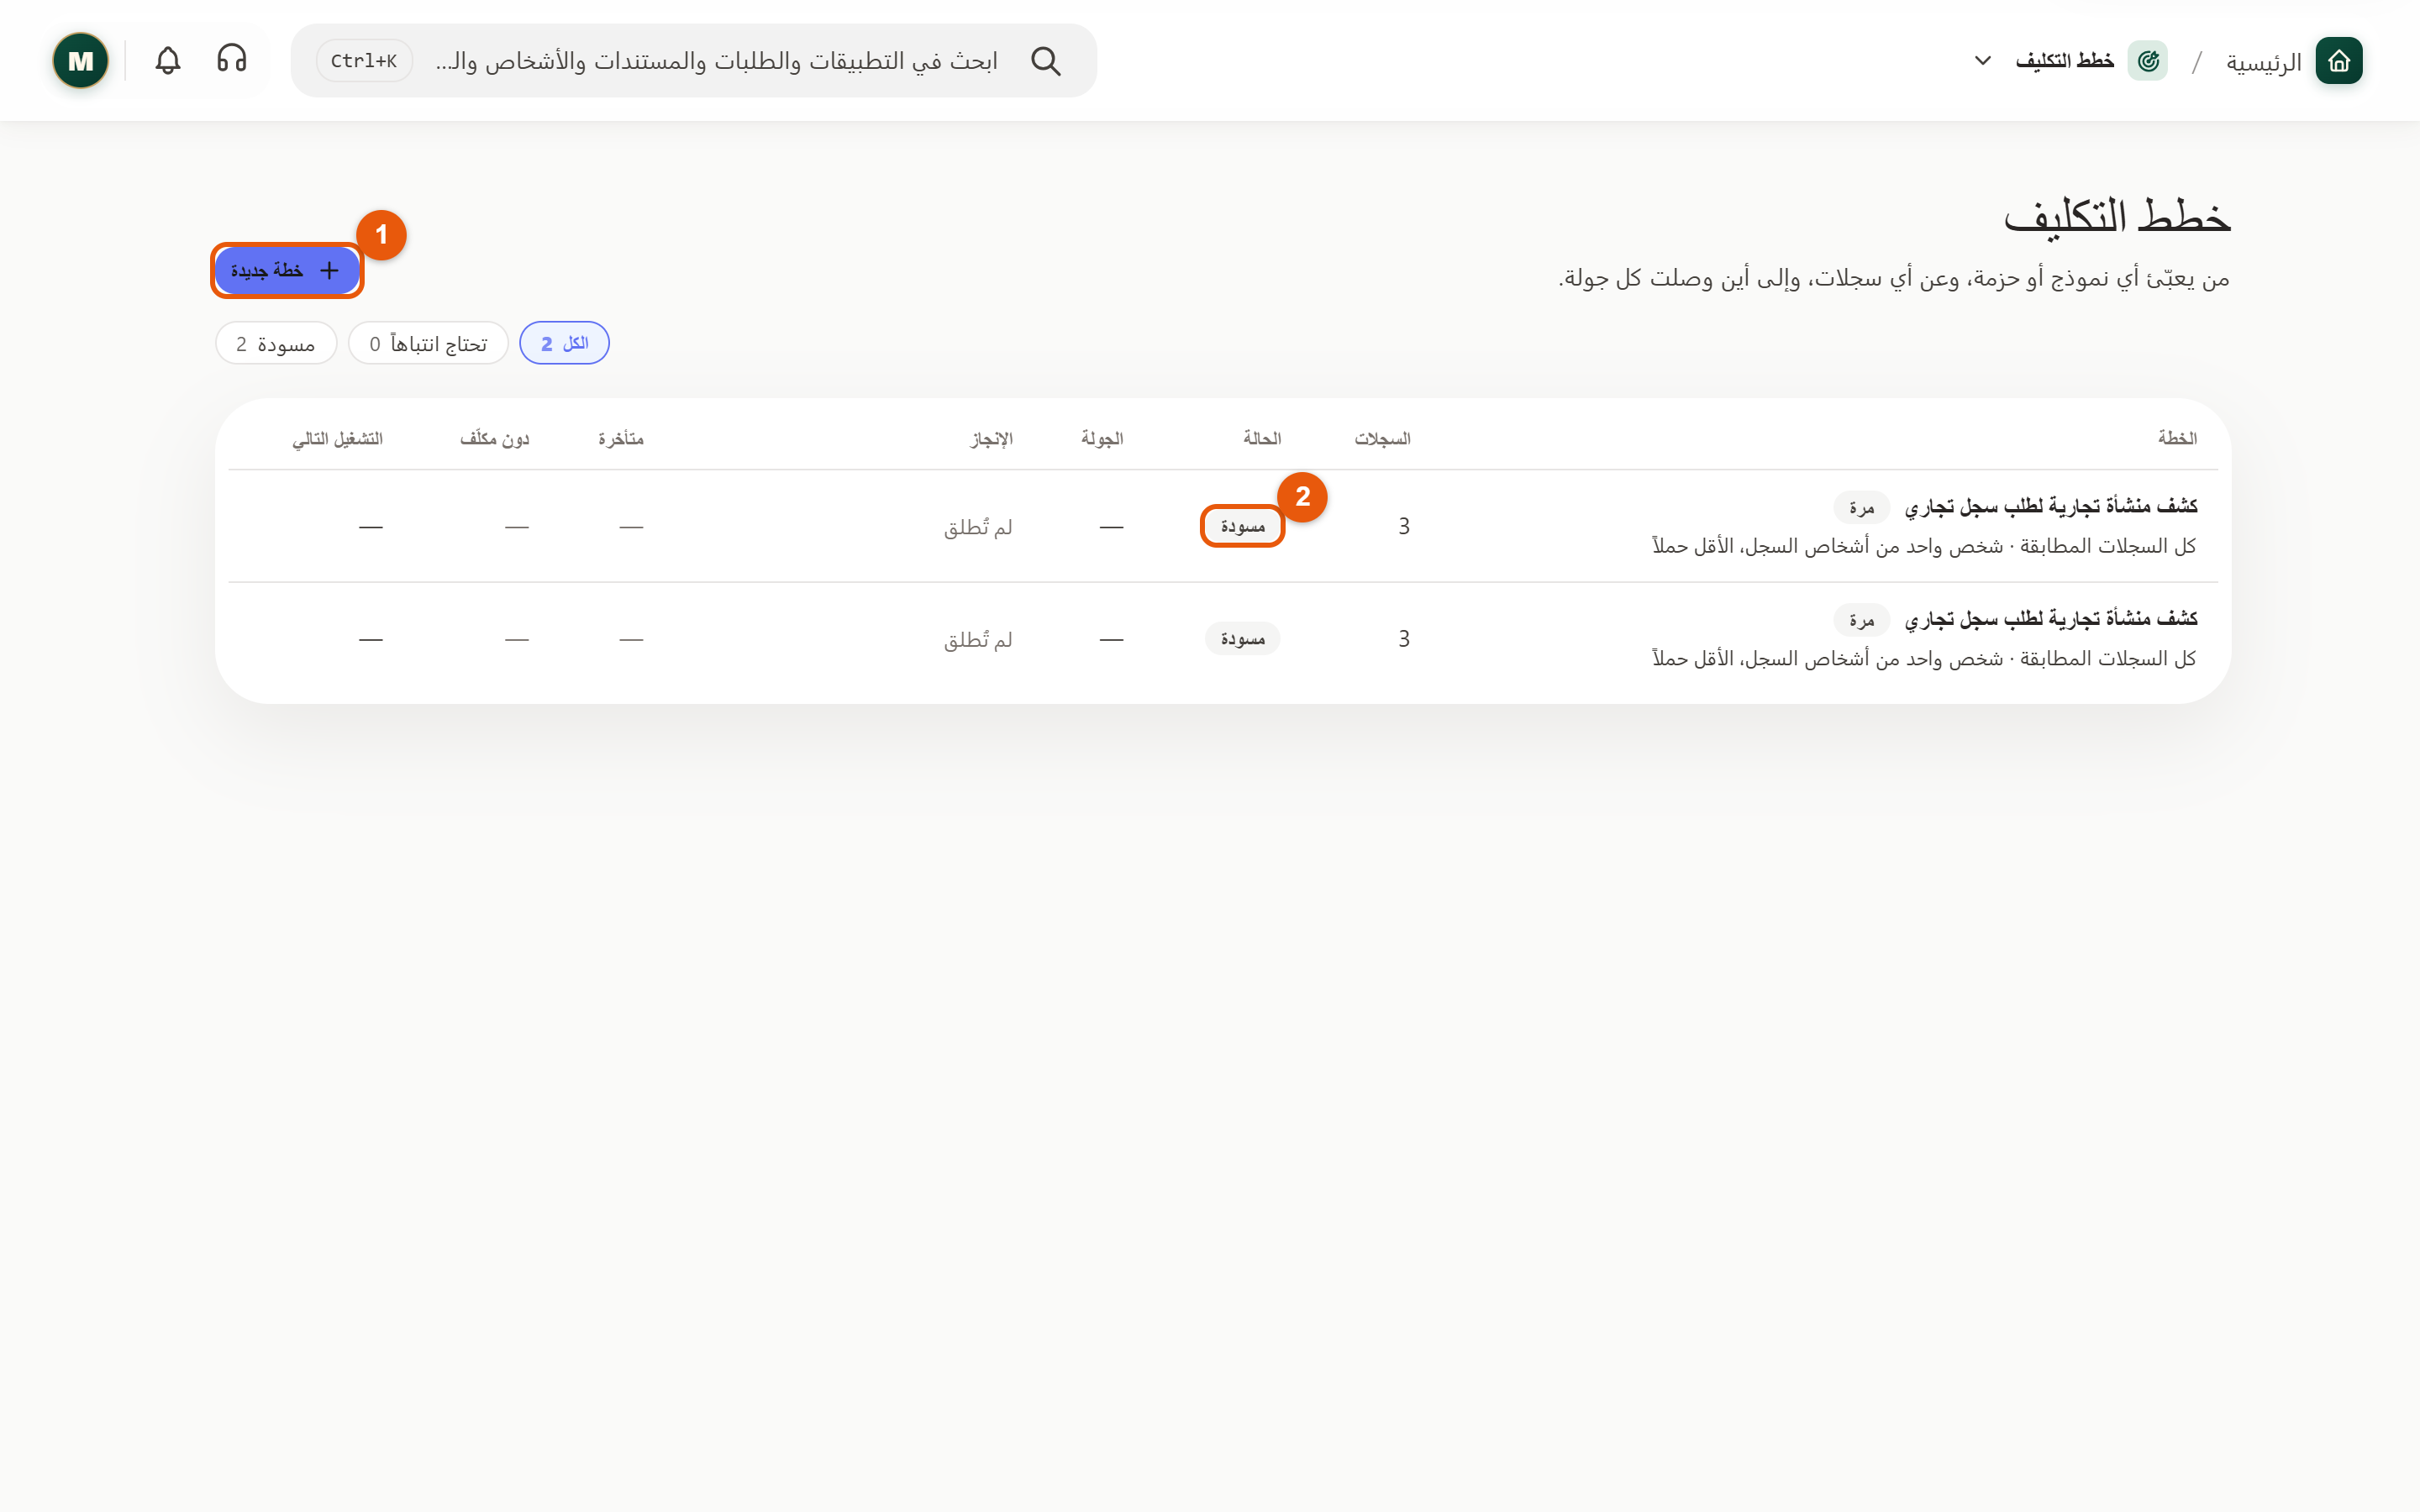
\includegraphics[width=0.95\linewidth]{assets/screens/plans-list.png}
\caption{من مسودة خطة إلى تكليف فعلي}
\label{fig:plans}
\shotnote{الخطة المحفوظة كمسودة لا تعني أن العمل وصل إلى الباحث. ① «خطة جديدة»: ابدأ إعداد الجولة. ② «مسودة»: أكمل الإعداد والمعاينة ثم أنشئ التكليفات لإطلاق العمل.}
\end{figure}

\textbf{تحقق:} لم تعد الخطة «مسودة» في «خطط التكليف»، ويظهر التكليف لنور في «تكليفات مطلوبة منك». إذا عرضت المعاينة «دون مرشح»، تأكد من تعيين نور النشط في منصب الباحث ومن اختيار هذا المنصب في الخطة.

\section{نفّذ الكشف وأرسله للتدقيق}
\label{sec:build-run}

\textbf{ماذا يفعل الباحث؟} يفتح نور المهمة، ويتأكد من المنشأة، ثم يسجل ما وجده في الزيارة. تحفظ الإجابة تفاصيل هذه الزيارة، بينما ينتظر تعديل ملف المنشأة قرار المدقق.

\begin{enumerate}
\item يدخل نور بحسابه ويفتح «تكليفات مطلوبة منك»، ثم يضغط «ابدأ» بجانب فرن الأمانة.
\item يتأكد من ظهور الفرن في سؤال المنشأة، ويقرأ البيانات التي جلبها النموذج.
\item يصحح البيانات التي تحتاج تصحيحاً، ويملأ نتيجة الكشف والتوصية، ويرفق المستندات المطلوبة.
\item يضغط «إرسال الطلب»، ثم يؤكد الإرسال. إذا ظهر تنبيه عن سؤال مطلوب، يكمله ثم يعيد الإرسال.
\end{enumerate}

\textbf{تحقق:} ينتقل الكشف إلى التدقيق وتظهر موافقته للمكلّف بها. يجب أن يبقى ملف المنشأة بقيمه السابقة إلى حين الاعتماد؛ تغيير إجابة العنوان وحده لا يعني تحديث الملف.

\section{اتخذ القرار وتأكد من النتيجة}
\label{sec:build-decision}

\textbf{ماذا تفعل المدققة؟} تراجع ريم الإجابة والمرفقات، ثم تختار قراراً. الإعادة تسمح لنور بالتصحيح، والرفض ينهي الكشف دون اعتماد، والموافقة تعتمد النتيجة وتطبق تحديثات المنشأة المسموح بها.

\begin{enumerate}
\item تدخل ريم بحسابها، وتفتح «موافقات بانتظارك»، ثم الكشف الخاص بفرن الأمانة.
\item تفتح الأقسام وتقرأ المرفقات. إذا كانت الخطوة تشترط قراءة جميع الأقسام، تكملها حتى تصبح أزرار القرار متاحة.
\item تختار «اعتماد الكشف» أو «رفض» أو «إعادة للتصحيح». تكتب سبب الرفض أو المطلوب استكماله، وتحدد الإقرار إذا ظهر، ثم تضغط «تأكيد».
\item عند الإعادة، يفتح نور الكشف نفسه ويكمل المطلوب ثم يعيد إرساله. لا ينشئ كشفاً بديلاً عن الإجابة المعادة.
\item عند الاعتماد، افتح ملف فرن الأمانة وتأكد من انتقال التصحيحات إلى الحقول المرتبطة.
\end{enumerate}

\textbf{تحقق:} اكتمل الكشف عندما أصبحت حالته «مقبول»، ووصلت التغييرات المسموح بها إلى ملف المنشأة. إذا ظهر في الكشف تنبيه «لم تُحفظ الإجابات في السجلات»، أو ظهر الزر «السجلات · لم تُحفظ»، فافتح «السجلات» واقرأ السبب المكتوب بعد «السبب:»، مثل «غير مسموح» أو «قيم غير صالحة». عالج السبب في إذن الكتابة أو في القيمة المرتبطة، ثم اضغط «اكتب مجدداً». القرار نفسه لا يتغير؛ ما يُعاد هو الكتابة إلى الملف فقط. سنعرض الآن بيانات المنشآت في لوحة مؤشرات.

\section{أنشئ لوحة مؤشرات المنشآت التجارية}
\label{sec:build-dashboard}

\textbf{لماذا؟} يحتاج أحمد إلى معرفة عدد المنشآت، وأين تقع، وما أنشطتها، ثم الوصول إلى منشأة محددة. «لوحة المؤشرات» تجمع هذه المعلومات في شاشة واحدة. سنجعلها تقرأ ملفات «المنشآت التجارية» التي جهزناها؛ فلا نكتب بيانات الفرن مرة أخرى داخل اللوحة.

\begin{enumerate}
\item افتح «ادوات البناء» ← «لوحات المعلومات» ← «إنشاء لوحة معلومات».
\item اكتب الاسم «مؤشرات المنشآت التجارية»، والوصف «متابعة المنشآت حسب المحافظة والنشاط والبحث عن منشأة».
\item اضغط «إنشاء». يفتح محرر اللوحة، وهو المكان الذي تضيف فيه الأرقام والرسوم والجدول.
\item سنضيف أربعة عناصر: رقم لعدد المنشآت، ورسم حسب المحافظة، ورسم حسب النشاط، وجدول يعرض تفاصيل المنشآت. ثم نضيف أدوات البحث والتصفية ونربطها بالعناصر الأربعة.
\end{enumerate}

توضح الصورة حقول البداية: اكتب الاسم عند ① والوصف عند ②، ثم اضغط «إنشاء» عند ③ للانتقال إلى المحرر. الوصف يشرح غرض اللوحة؛ لا يحدد مصدر بياناتها، فهذا تضبطه داخل كل عنصر.

\begin{figure}[H]
\centering
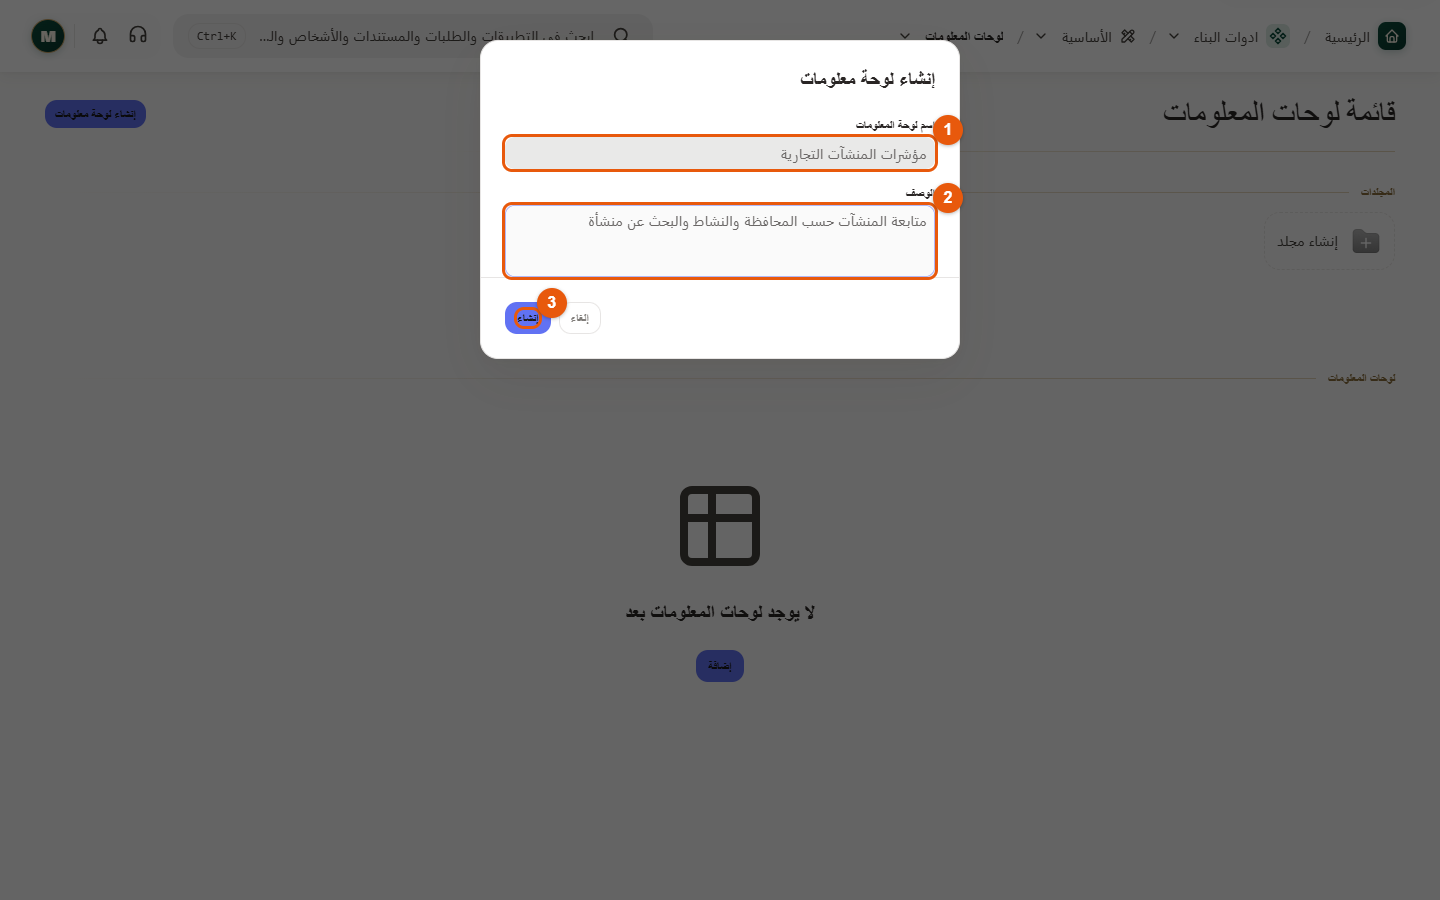
\includegraphics[width=0.95\linewidth]{assets/screens/org-dashboard-create.png}
\caption{إنشاء لوحة مؤشرات المنشآت التجارية}
\label{fig:dashboard-create}
\shotnote{① اسم اللوحة الذي سيظهر للفريق. ② وصف قصير لما سيجده المشاهد. ③ إنشاء اللوحة وفتح محررها. هذه شاشة إدخال قبل الإنشاء، وليست لوحة منشورة.}
\end{figure}

\textbf{تحقق:} يظهر اسم اللوحة في المحرر. إنشاء اللوحة وحده لا يجلب بيانات؛ سنحدد مصدر كل عنصر في الخطوات التالية.

\subsection{خطط للوحة قبل إضافة عناصرها}

\begin{table}[H]
\centering
\caption{السؤال الذي يجيب عنه كل عنصر}
\label{tab:dashboard-design}
\begin{tabularx}{\linewidth}{Y Y Y}
\rcHeaderRow
\thh{سؤال أحمد} & \thh{العنصر المناسب} & \thh{الإعداد الذي يجيب عنه}\\
كم منشأة تطابق اختياراتي؟ & مؤشر «عدد المنشآت». & مصدر المنشآت التجارية وتجميع العدد.\\
كيف تتوزع حسب المحافظة؟ & رسم أعمدة. & الفئة: المحافظة؛ القيمة: عدد السجلات.\\
ما الأنشطة التي تغطيها؟ & رسم حسب النشاط. & الفئة: النشاط؛ القيمة: عدد السجلات.\\
ما أسماء هذه المنشآت وبياناتها؟ & جدول التفاصيل. & نفس المصدر، مع حقول الاسم والنشاط والمحافظة والعنوان.\\
كيف أصل إلى منشأة محددة؟ & محدد يبحث في المنشآت. & اختيار ملف ثم تصفية العناصر بمعرّفه.\\
\end{tabularx}
\end{table}

كل صف في مصدرنا يمثل منشأة واحدة. هذا مهم للحساب: المؤشر يعدّ ملفات المنشآت حتى لو كان لكل منها عدة كشوف. إذا أردت لاحقاً قياس عدد الكشوف أو مدة تدقيقها فحدد مصدر إجابات الكشف وحقوله أولاً؛ تغيير عنوان مؤشر المنشآت إلى «الكشوف» لا يغير ما يعدّه.

رتب اللوحة من الإجمال إلى التفاصيل: المؤشر أعلى الصفحة، ثم الرسمان، ثم الجدول. اجعل العنوان يصف الرقم كما سيُستخدم؛ سميناه «عدد المنشآت» لأنه يتغير مع المرشحات، وليس إجمالياً ثابتاً للمؤسسة.

\section{اربط مؤشر العدد بالمنشآت}
\label{sec:build-kpi}

\textbf{ما معنى مؤشر أداء؟} هو رقم يجيب عن سؤال محدد. سؤالنا هنا: كم منشأة لدينا؟ مصدر هذا الرقم هو «المنشآت التجارية». أما «التجميع» فيحدد طريقة الحساب؛ سنختار «العدد» لعدّ الملفات.

\begin{enumerate}
\item اضغط «مؤشر أداء» من شريط إضافة العناصر.
\item في إعدادات العنصر افتح «البيانات» ← «القيمة». اختر مصدر البيانات «كيان»، ثم «المنشآت التجارية». كلمة «كيان» هنا تعني نوع السجلات الذي سيقرأه المؤشر.
\item اختر «العدد» في «التجميع». لا تحتاج إلى حقل رقمي؛ المطلوب عدّ المنشآت نفسها.
\item افتح «عام»، واكتب العنوان «عدد المنشآت»، ثم أغلق إعدادات العنصر واضغط «حفظ».
\end{enumerate}

\textbf{تحقق:} إذا أضفت في الخطوات السابقة فرن الأمانة وحده، فالعدد المتوقع 1. هذا عدد المنشآت، وليس عدد زيارات الكشف؛ إجراء كشفين على الفرن لا يجعله منشأتين.

\subsection{اختر طريقة الحساب عن فهم}

«العدد» يعدّ السجلات، و«المجموع» يجمع قيماً في حقل رقمي، و«المتوسط» يقسم مجموع القيم الداخلة في الحساب على عددها. لذلك نختار العدد هنا؛ لا نجمع أرقام السجل التجاري، ولا نعاملها كقياس كمي. إذا استخدمت لاحقاً حقلاً رقمياً، حدد الحقل ووحدته وما تعنيه القيمة الفارغة قبل اختيار التجميع.

\begin{enumerate}
\item أعد فتح «البيانات» في مؤشر العدد. راجع المصدر أولاً، ثم نوع السجلات، ثم التجميع، ثم المرشحات. هذه الإعدادات تفسر الرقم قبل التنسيق والألوان.
\item افتح «عام»، واضبط العنوان والعرض والارتفاع بحيث يظهر الرقم كاملاً. لا تضف وحدة قياس مالية أو نسبة إلى عدد المنشآت.
\item احفظ ثم أعد فتح إعدادات المؤشر. تأكد أن مصدره ما زال «المنشآت التجارية»، وأنك لم تترك بيانات عرض تجريبية بدلاً منه.
\end{enumerate}

\textbf{تحقق:} تستطيع تفسير المؤشر بهذه الجملة: «يعد هذا الرقم سجلات المنشآت التجارية المسموح للمشاهد بقراءتها والتي تطابق المرشحات الحالية». إذا لم يطابق القائمة، راجع المصدر والصلاحيات والمرشحات قبل افتراض خطأ في الجمع.

\section{أضف توزيع المنشآت وجدول التفاصيل}
\label{sec:build-charts}

\textbf{لماذا؟} الرقم يوضح الإجمالي، والرسم يوضح توزيعه، والجدول يبين الملفات التي جاء منها. «حقل الفئة» هو ما نقسم المنشآت بحسبه، مثل المحافظة أو النشاط.

\begin{enumerate}
\item اضغط «إضافة رسم بياني (Nivo)»، واختر رسم «أعمدة».
\item في «البيانات» اختر «كيان» ← «المنشآت التجارية». اختر «المحافظة» في «حقل الفئة»، و«عدد» في «نوع القيمة». بذلك يمثل كل عمود عدد المنشآت في محافظة.
\item في «عام» سمِّ الرسم «المنشآت حسب المحافظة».
\item أضف رسماً ثانياً بالطريقة نفسها، واجعل «حقل الفئة» هو «النشاط»، وسمِّه «المنشآت حسب النشاط».
\item اضغط «جدول». اختر مصدر «كيان» ← «المنشآت التجارية»، ثم في «اختر الحقول» حدد اسم المنشأة، والنشاط، والمحافظة، والعنوان التفصيلي.
\item سمِّ الجدول «تفاصيل المنشآت»، ثم اضغط «حفظ» للوحة.
\end{enumerate}

\textbf{تحقق:} يظهر فرن الأمانة في الجدول، ويُحسب ضمن محافظته ونشاطه في الرسمين. بعد اعتماد تصحيح عنوانه في الكشف وتحديث اللوحة، يظهر العنوان المصحح؛ لأن الجدول يقرأ ملف المنشأة الذي حدّثه الكشف.

\subsection{افهم الفئة والقيمة وحدّ الصفوف}

في رسم المحافظة، الفئة هي اسم المحافظة والقيمة هي عدد المنشآت فيها. لو اخترت «اسم المنشأة» فئةً، فستحصل على عمود لكل منشأة، ولن يجيب الرسم عن التوزيع الجغرافي. اختر الفئة أولاً ثم راجع إعداد القيمة؛ تغيير الفئة قد يستلزم إعادة تحديد حقل القيمة في الرسوم التي تقيس حقلاً رقمياً.

للرسم الدائري فائدة عندما تريد نسب التوزيع على عدد قليل من الأنشطة. اختر مصدر المنشآت وحقل فئة النشاط؛ أما مقارنة محافظات كثيرة فالأعمدة أسهل قراءة. لا تستنتج من غياب فئة أن عددها صفر قبل التأكد من بيانات الحقل والمرشحات.

\begin{enumerate}
\item افتح جدول التفاصيل وراجع «اختر الحقول». ضع اسم المنشأة أولاً، ثم المحافظة والنشاط والعنوان. استخدم الجدول لمراجعة الملفات، لا لإعادة حساب بيانات مختلفة عن المؤشر.
\item راجع «حد الصفوف» في إعدادات الجدول. هذا يحد كمية التفاصيل المعروضة؛ لا تفترض أن عدد الصفوف الظاهرة يساوي جميع النتائج.
\item اختر محافظة من اللوحة، ثم افحص قيم المحافظة في الجدول. يجب ألا ترى ملفاً من محافظة أخرى بعد ربط المرشح.
\item افحص السجلات ذات المحافظة أو النشاط الفارغ. أكمل بياناتها عند الحاجة؛ لا تنسبها إلى محافظة أو نشاط بافتراض من عندك.
\end{enumerate}

\textbf{تحقق:} عند مقارنة مجموع الأعمدة بالمؤشر، استخدم المصدر والصلاحيات والمرشحات نفسها، وتحقق من معالجة القيم الفارغة وحدود عرض الفئات. وعند مقارنة الجدول، راجع جميع الصفوف أو الصفحات الداخلة في المقارنة.

\section{أضف التصفية بالمحافظة والنشاط واربطها بالعناصر}
\label{sec:build-dashboard-filters}

\textbf{لماذا؟} قد يريد أحمد رؤية منشآت محافظة واحدة فقط. «المرشح» هو شرط يضيّق النتائج. سننشئ قائمة لاختيار المحافظة، ثم نخبر كل عنصر أي حقل يجب أن يقارنه بهذا الاختيار. ظهور القائمة وحده لا يكفي لربطها بالمؤشرات.

\begin{enumerate}
\item افتح إعداد «المرشحات» في محرر اللوحة، وأضف مرشحاً. اختر النوع «اختر الحقل»، واكتب التسمية «المحافظة».
\item اجعل «النطاق» هو «لوحة التحكم كاملة». في «مصدر الخيارات» اختر «من حقل كيان»، ثم اختر حقل «المحافظة» من «المنشآت التجارية». هكذا تأتي أسماء المحافظات من خيارات الحقل نفسه.
\item احفظ إعداد المرشح، ثم افتح إعدادات عنصر «عدد المنشآت» ← «البيانات» ← «المرشحات» ← «تكوين مرشحات البيانات» ← «إضافة تصفية».
\item اختر حقل «المحافظة» والشرط «يساوي». بجانب خانة القيمة اضغط زر «استخدام في المرشح»، واختر «المحافظة». يضيف النظام مرجع الاختيار؛ لا تكتب اسم محافظة ثابتاً في هذه الخانة.
\item كرر هذا الربط في رسم المحافظة، ورسم النشاط، وجدول التفاصيل. بهذه الخطوة تعتمد العناصر الأربعة على اختيار المحافظة نفسه.
\item أضف مرشحاً ثانياً اسمه «النشاط» من النوع «اختر الحقل»، ومصدر خياراته حقل «النشاط» من «المنشآت التجارية».
\item في كل عنصر أضف شرطاً آخر: حقل «النشاط» «يساوي» مرشح «النشاط»، باستخدام الزر نفسه. اجعل جمع الشرطين «و» حتى تعرض النتائج التي تطابق المحافظة والنشاط معاً، ثم احفظ.
\end{enumerate}

\textbf{تحقق:} اختر محافظة الفرن ونشاطه؛ يجب أن يظهر في الجدول ويُحسب في المؤشر. اختر محافظة أخرى فلا يظهر. اضغط «مسح الكل» لإعادة عرض جميع المنشآت المتاحة. إذا تغير الجدول وحده، أكمل ربط المرشحين ببقية العناصر.

\subsection{ميّز المرشح الثابت عن اختيار المشاهد}

المرشح الثابت يضعه المصمم داخل عنصر، مثل حصر مؤشر بنشاط معين دائماً. أما مرشح المشاهد فهو قيمة يغيرها أحمد أثناء القراءة. عندما تستخدم زر «استخدام في المرشح» فأنت تربط شرط العنصر بتلك القيمة المتغيرة. المرجع الذي يضيفه النظام يبدأ بـ\en{$selector:}؛ لا تستبدله بنص اسم القائمة أو باسم محافظة.

إذا احتجت مؤشراً ثابتاً لنشاط الفرن، أضف مؤشراً بعنوان يوضح ذلك، واختر مصدر المنشآت وتجميع العدد، ثم أضف شرط النشاط «يساوي» خيار نشاط الفرن. إذا كانت خانة القيمة تطلب القيمة الخام، انسخ مفتاح الخيار من إعداد الحقل. هذا إعداد مختلف عن ربطه بقائمة النشاط؛ «مسح الكل» يمسح اختيارات المشاهد، ولا يحذف شرطاً ثابتاً وضعته داخل العنصر.

«و» تعني تحقق الشرطين معاً: المحافظة المختارة والنشاط المختار. أما «أو» فتعني تحقق أحدهما، وقد تعرض منشآت من محافظات أخرى لأنها تطابق النشاط. استخدم «و» في لوحة المثال. والنطاق يحدد العناصر التي يمكن أن يتأثر بها المرشح، لكنه لا يعوض اختيار حقل صحيح وربط قيمته داخل العنصر.

\textbf{تحقق:} افتح إعدادات العناصر الأربعة واحداً واحداً: يجب أن يقرأ شرط المحافظة مرشح المحافظة، وشرط النشاط مرشح النشاط. إذا كان أحدها يحمل قيمة ثابتة أو مرجع القائمة الأخرى فلن تتطابق النتائج.

\section{أضف البحث عن منشأة واربط الاختيار باللوحة}
\label{sec:build-dashboard-search}

\textbf{ما الفرق بين البحث والتصفية؟} البحث بالاسم يساعدك على العثور على منشأة بعينها، مثل فرن الأمانة. أما اختيار المحافظة أو النشاط فيجمع منشآت لها الصفة نفسها. سنضيف «محدد» منشأة: قائمة تبحث فيها بالاسم، ثم تختار النتيجة لعرض بياناتها في اللوحة.

\begin{enumerate}
\item افتح إعداد «المرشحات»، وأضف مرشحاً من النوع «محدد». اكتب التسمية «ابحث عن منشأة»، واختر الكيان «المنشآت التجارية».
\item اجعل نطاقه «لوحة التحكم كاملة»، واترك القيمة الافتراضية فارغة و«مطلوب» غير مفعّل، ثم احفظ. بذلك يمكن للمشاهد عرض جميع المنشآت أو اختيار واحدة.
\item افتح إعدادات جدول التفاصيل ← «البيانات» ← «المرشحات» ← «تكوين مرشحات البيانات»، وأضف تصفية.
\item اختر الحقل «المعرف» والشرط «يساوي». اضغط «استخدام في المرشح» بجانب القيمة، واختر «ابحث عن منشأة». المعرف يميز ملف المنشأة حتى لو تشابه اسمان؛ والمحدد يرسل معرف الملف المختار تلقائياً.
\item أضف الربط نفسه إلى مؤشر العدد والرسمين، مع إبقاء شروط المحافظة والنشاط متصلة بـ«و»، ثم اضغط «حفظ».
\item في عرض اللوحة افتح «ابحث عن منشأة»، واكتب «الأمانة»، ثم اختر «فرن الأمانة» من النتائج. كتابة الكلمة تبحث في قائمة الاختيار؛ اختيار النتيجة هو الذي يصفّي عناصر اللوحة.
\end{enumerate}

\textbf{تحقق:} بعد مسح المرشحات الأخرى واختيار الفرن، يعرض الجدول ملفه ويصبح عدد المنشآت 1. امسح اختيار المنشأة لعرض الجميع. إذا جمعت اختياره مع محافظة لا ينتمي إليها، فالنتيجة صفر لأن الشرطين لا ينطبقان معاً.

\subsection{اختبر البحث والربط خطوة خطوة}

\begin{enumerate}
\item امسح جميع الاختيارات، وافتح محدد المنشأة. ابحث بجزء من الاسم «الأمانة»؛ البحث هنا يستهدف الاسم المعروض للسجل، وليس كل كلمات الملاحظات والعنوان.
\item اختر النتيجة، ثم افحص الجدول أولاً. إذا ظهر الفرن وحده، افحص المؤشر والرسمين. إذا بقي أحدها يعرض الجميع فراجع شرط «المعرف» في ذلك العنصر تحديداً.
\item امسح الاختيار من المحدد. يجب أن تعود النتائج المتاحة وفق المرشحات الأخرى، إن بقيت مختارة.
\item اختر الفرن ومحافظة مختلفة عن محافظته. النتيجة الفارغة متوقعة. امسح المحافظة وحدها وتأكد من عودة الفرن؛ بهذه التجربة تميز التعارض الصحيح بين الشروط عن فشل جلب البيانات.
\end{enumerate}

\textbf{تحقق:} تعرف الآن الفرق بين عدم وجود نتيجة في قائمة البحث، وعدم ظهور بيانات بعد الاختيار. الأولى تستدعي مراجعة الاسم والمصدر وصلاحية القراءة؛ والثانية تستدعي مراجعة معرف المنشأة وربط العناصر وبقية المرشحات.

\section{انشر اللوحة وجرّب البحث بحساب رئيس الفريق}
\label{sec:build-dashboard-publish}

\textbf{لماذا؟} الحفظ يحتفظ بإعداد اللوحة، والنشر يتيح نسختها للمشاهدين. يحتاج أحمد إلى صلاحية مشاهدة اللوحة وقراءة المنشآت التي تُحسب منها النتائج.

\begin{enumerate}
\item افتح «الإعدادات» في اللوحة، وفعّل «إظهار في التنقل». اختر تطبيق «حماية المستهلك» وقسم «السجلات».
\item اختر «بصلاحيات المشاهد» في «البيانات المعروضة»، ثم احفظ. تعرض اللوحة لكل شخص البيانات المسموح له بقراءتها.
\item افتح «إدارة الوصول»، واختر المنصب «رئيس فريق الكشف الميداني — 01»، وامنحه مستوى «مشاهد». هذا المستوى يسمح بفتح اللوحة دون تعديل إعدادها.
\item في صلاحيات «المنشآت التجارية»، امنح رئيس الفريق «قائمة» و«فتح» من خلال الدور المسند إليه. مشاركة اللوحة لا تمنح قراءة سجلاتها تلقائياً.
\item اضغط «حفظ» ثم «نشر». ادخل بحساب أحمد وافتح «حماية المستهلك» ثم لوحة «مؤشرات المنشآت التجارية» من قسمها.
\item جرّب ثلاث عمليات بالترتيب: اعرض الجميع، ثم صفِّ حسب المحافظة والنشاط، ثم امسح المرشحات وابحث عن فرن الأمانة واختره. في كل مرة قارن مؤشر العدد بالمنشآت المطابقة في الجدول، مع الانتباه إلى الصفحات وحدّ الصفوف المعروضة.
\end{enumerate}

\textbf{تحقق:} يستطيع أحمد فتح اللوحة والبحث والتصفية، وتتغير العناصر الأربعة معاً. إذا لم تظهر البيانات، راجع صلاحية قراءة المنشآت. وإذا بقيت إعدادات قديمة، انشر آخر تعديل. صار تسلسل العمل مكتملاً: ملف منشأة ← كشف واعتماد ← تحديث الملف ← متابعة وبحث في اللوحة.

\subsection{شخّص المشكلة من موضعها}

\begin{table}[H]
\centering
\caption{أعراض شائعة وما تفحصه أولاً}
\label{tab:builder-diagnosis}
\begin{tabularx}{\linewidth}{Y Y}
\rcHeaderRow
\thh{ما الذي تراه؟} & \thh{الفحص والإصلاح}\\
المنشأة لا تظهر في سؤال السجل & راجع نوع السجلات وصلاحية القائمة والفتح واسم السجل المعروض.\\
تظهر المنشأة لكن عنوانها لا يُجلب & راجع قيمة العنوان في الملف، ثم حقل الربط واتجاه القراءة.\\
لا يمكن إرسال الكشف & افتح تنبيه السؤال المطلوب أو القاعدة؛ تأكد أن السؤال المطلوب ظاهر وقابل للإجابة.\\
لا يصل قرار التدقيق إلى ريم & راجع حالة الكشف وتشغيل خطوة الموافقة والمنصب وشاغله النشط.\\
بطاقة الربط تعرض «بانتظار موافقة مسؤول» & لم يُسمح للنموذج بالكتابة بعد؛ يوافق مسؤول «المنشآت التجارية» على الطلب، ثم تتحقق من «مسموح».\\
معاينة الخطة تعرض «دون مرشح» & راجع تعيين نور النشط في منصب الباحث، واختيار هذا المنصب في «المرشحون».\\
لا يظهر التكليف لنور & تأكد أنك ضغطت «إنشاء التكليفات»؛ الخطة التي بقيت «مسودة» لم تُرسل أي عمل.\\
الكشف مقبول والملف لم يتغير & اقرأ نتيجة تطبيق السجلات؛ راجع إذن الكتابة والحقول والقيم، ولا تساوِ بين نجاح القرار ونجاح الكتابة.\\
القائمة موجودة ولا تغير اللوحة & راجع نطاقها وربط قيمتها داخل كل عنصر.\\
اللوحة صفر بعد اختيار عدة مرشحات & امسحها وأعد واحداً واحداً؛ قد لا يوجد سجل يحقق الشروط مجتمعة.\\
المسؤول يرى بيانات وأحمد لا يراها & قارن صلاحيات قراءة المنشآت ومشاركة اللوحة، لا شكل العنصر فقط.\\
الجدول أقصر من رقم المؤشر & راجع حد الصفوف والصفحات، ثم تطابق مصدر البيانات والمرشحات.\\
التعديل يظهر في المحرر فقط & احفظ وانشر، ثم افتح النسخة المنشورة من حساب المشاهد.\\
\end{tabularx}
\end{table}

\subsection{تطبيق أخير لتتأكد أنك فهمت أدوات البناء}

نفّذ دورة كاملة دون الرجوع إلى أسماء الأزرار فقط: اختر الفرن، وصحح عنوانه في كشف، وأعده للتصحيح مع تعليق، ثم أرسله واعتمده. ابحث عنه في اللوحة وتأكد من العنوان الجديد، وجرّب المحافظة والنشاط ومسح المرشحات. بعد ذلك اشرح لماذا لم يتغير عدد المنشآت رغم إضافة كشف جديد.

\textbf{تحقق:} تستطيع تحديد مكان كل إعداد وتفسير أثره: السؤال يجمع الإجابة، والربط يحدد ملفها وحقولها، والقاعدة تتحقق منها، والمسار يوجه القرار، والصلاحية تسمح بالفعل، والعنصر يحسب البيانات، والمرشح يحدد الجزء المعروض. إذا أخفقت تجربة، ارجع إلى الجزء المسؤول عنها وأعدها بعد التصحيح؛ هذا هو معيار إتقان التطبيق.
